%%%%%%%%%%%%%%%%%%%%%%%%%%%%%%%%%%%%%%%%%
% Beamer Presentation
% LaTeX Template
% Version 2.0 (March 8, 2022)
%
% This template originates from:
% https://www.LaTeXTemplates.com
%
% Author:
% Vel (vel@latextemplates.com)
%
% License:
% CC BY-NC-SA 4.0 (https://creativecommons.org/licenses/by-nc-sa/4.0/)
%
%%%%%%%%%%%%%%%%%%%%%%%%%%%%%%%%%%%%%%%%%

%----------------------------------------------------------------------------------------
%	PACKAGES AND OTHER DOCUMENT CONFIGURATIONS
%----------------------------------------------------------------------------------------

\documentclass[
	14pt, % Set the default font size, options include: 8pt, 9pt, 10pt, 11pt, 12pt, 14pt, 17pt, 20pt
	%t, % Uncomment to vertically align all slide content to the top of the slide, rather than the default centered
	aspectratio=169, % Uncomment to set the aspect ratio to a 16:9 ratio which matches the aspect ratio of 1080p and 4K screens and projectors
]{beamer}
\usepackage[absolute,overlay]{textpos}
\usepackage{graphicx, makecell, setspace, tikz}
\usetikzlibrary{positioning,calc}

\graphicspath{{Images/}{./}} % Specifies where to look for included images (trailing slash required)

\usepackage{booktabs} % Allows the use of \toprule, \midrule and \bottomrule for better rules in tables

%----------------------------------------------------------------------------------------
%	SET CHINESE FONT
%----------------------------------------------------------------------------------------

\usepackage{ctex}
\setCJKmainfont[BoldFont=STSong, ItalicFont=STKaiti]{STSong} % useless in beamer
\setCJKsansfont[BoldFont=STHeiti, ItalicFont=STKaiti]{STSong}
\setCJKmonofont{STFangsong}

%----------------------------------------------------------------------------------------
%	SET VARIABLE BLOCK
%----------------------------------------------------------------------------------------

\newenvironment<>{varblock}[2][1\textwidth]{%
  \setlength{\textwidth}{#1}
  \begin{actionenv}#3%
    \def\insertblocktitle{#2}%
    \par%
    \usebeamertemplate{block begin}}
  {\par%
    \usebeamertemplate{block end}%
  \end{actionenv}}
  
%----------------------------------------------------------------------------------------
%	SET LINE SPACING 
%----------------------------------------------------------------------------------------

\linespread{1.1} % Adjust line spacing

%----------------------------------------------------------------------------------------
%	SET FRAME TITLE
%----------------------------------------------------------------------------------------

\setlength{\parskip}{0.5ex}
\addtobeamertemplate{frametitle}{\vskip-0.9ex}{\vspace{0em}} % {}{adjust the height of frame title}{adjust the position of body paragraph}
%\setbeamertemplate{frametitle}{%
%    \nointerlineskip%
%    \begin{beamercolorbox}[wd=\paperwidth,ht=2.0ex,dp=0.6ex]{frametitle}
%        \hspace*{1ex}\insertframetitle%
%    \end{beamercolorbox}%
%}

%----------------------------------------------------------------------------------------
%	SELECT LAYOUT THEME
%----------------------------------------------------------------------------------------

% Beamer comes with a number of default layout themes which change the colors and layouts of slides. Below is a list of all themes available, uncomment each in turn to see what they look like.

%\usetheme{default}
%\usetheme{AnnArbor}
%\usetheme{Antibes}
%\usetheme{Bergen}
%\usetheme{Berkeley}
%\usetheme{Berlin}
%\usetheme{Boadilla}
%\usetheme{CambridgeUS}
%\usetheme{Copenhagen}
%\usetheme{Darmstadt}
%\usetheme{Dresden}
%\usetheme{Frankfurt}
%\usetheme{Goettingen}
%\usetheme{Hannover}
%\usetheme{Ilmenau}
%\usetheme{JuanLesPins}
%\usetheme{Luebeck}
\usetheme{Madrid}
%\usetheme{Malmoe}
%\usetheme{Marburg}
%\usetheme{Montpellier}
%\usetheme{PaloAlto}
%\usetheme{Pittsburgh}
%\usetheme{Rochester}
%\usetheme{Singapore}
%\usetheme{Szeged}
%\usetheme{Warsaw}

%----------------------------------------------------------------------------------------
%	SELECT COLOR THEME
%----------------------------------------------------------------------------------------

% Beamer comes with a number of color themes that can be applied to any layout theme to change its colors. Uncomment each of these in turn to see how they change the colors of your selected layout theme.

%\usecolortheme{albatross}
%\usecolortheme{beaver}
%\usecolortheme{beetle}
%\usecolortheme{crane}
%\usecolortheme{dolphin}
%\usecolortheme{dove}
%\usecolortheme{fly}
%\usecolortheme{lily}
%\usecolortheme{monarca}
%\usecolortheme{seagull}
%\usecolortheme{seahorse}
%\usecolortheme{spruce}
%\usecolortheme{whale}
%\usecolortheme{wolverine}

%----------------------------------------------------------------------------------------
%	SELECT FONT THEME & FONTS
%----------------------------------------------------------------------------------------

% Beamer comes with several font themes to easily change the fonts used in various parts of the presentation. Review the comments beside each one to decide if you would like to use it. Note that additional options can be specified for several of these font themes, consult the beamer documentation for more information.

\usefonttheme{default} % Typeset using the default sans serif font
%\usefonttheme{serif} % Typeset using the default serif font (make sure a sans font isn't being set as the default font if you use this option!)
%\usefonttheme{structurebold} % Typeset important structure text (titles, headlines, footlines, sidebar, etc) in bold
%\usefonttheme{structureitalicserif} % Typeset important structure text (titles, headlines, footlines, sidebar, etc) in italic serif
%\usefonttheme{structuresmallcapsserif} % Typeset important structure text (titles, headlines, footlines, sidebar, etc) in small caps serif

%------------------------------------------------

%\usepackage{mathptmx} % Use the Times font for serif text
\usepackage{palatino} % Use the Palatino font for serif text

%\usepackage{helvet} % Use the Helvetica font for sans serif text
\usepackage[default]{opensans} % Use the Open Sans font for sans serif text
%\usepackage[default]{FiraSans} % Use the Fira Sans font for sans serif text
%\usepackage[default]{lato} % Use the Lato font for sans serif text

%----------------------------------------------------------------------------------------
%	SELECT INNER THEME
%----------------------------------------------------------------------------------------

% Inner themes change the styling of internal slide elements, for example: bullet points, blocks, bibliography entries, title pages, theorems, etc. Uncomment each theme in turn to see what changes it makes to your presentation.

%\useinnertheme{default}
\useinnertheme{circles}
%\useinnertheme{rectangles}
%\useinnertheme{rounded}
%\useinnertheme{inmargin}

%----------------------------------------------------------------------------------------
%	SELECT OUTER THEME
%----------------------------------------------------------------------------------------

% Outer themes change the overall layout of slides, such as: header and footer lines, sidebars and slide titles. Uncomment each theme in turn to see what changes it makes to your presentation.

%\useoutertheme{default}
%\useoutertheme{infolines}
%\useoutertheme{miniframes}
%\useoutertheme{smoothbars}
%\useoutertheme{sidebar}
%\useoutertheme{split}
%\useoutertheme{shadow}
%\useoutertheme{tree}
%\useoutertheme{smoothtree}

%\setbeamertemplate{footline} % Uncomment this line to remove the footer line in all slides
%\setbeamertemplate{footline}[page number] % Uncomment this line to replace the footer line in all slides with a simple slide count

%\setbeamertemplate{navigation symbols}{} % Uncomment this line to remove the navigation symbols from the bottom of all slides

%----------------------------------------------------------------------------------------
%	PRESENTATION INFORMATION
%----------------------------------------------------------------------------------------

\title[基于深度学习的图像质量增强方法研究]{\textbf{基于深度学习的图像质量增强方法研究}} % The short title in the optional parameter appears at the bottom of every slide, the full title in the main parameter is only on the title page

%\subtitle{Optional Subtitle} % Presentation subtitle, remove this command if a subtitle isn't required

\author[黄昱博]{黄昱博} % Presenter name(s), the optional parameter can contain a shortened version to appear on the bottom of every slide, while the main parameter will appear on the title slide

\institute[北京邮电大学]{北京邮电大学 \\ \smallskip \textit{huangyubo@bupt.edu.cn}} % Your institution, the optional parameter can be used for the institution shorthand and will appear on the bottom of every slide after author names, while the required parameter is used on the title slide and can include your email address or additional information on separate lines

\date[\today]{硕士学位论文答辩 \\ \today} % Presentation date or conference/meeting name, the optional parameter can contain a shortened version to appear on the bottom of every slide, while the required parameter value is output to the title slide

%----------------------------------------------------------------------------------------

\begin{document}

%----------------------------------------------------------------------------------------
%	TITLE SLIDE
%----------------------------------------------------------------------------------------

\begin{frame}
	\titlepage % Output the title slide, automatically created using the text entered in the PRESENTATION INFORMATION block above
\end{frame}

%----------------------------------------------------------------------------------------
%	TABLE OF CONTENTS SLIDE
%----------------------------------------------------------------------------------------

% The table of contents outputs the sections and subsections that appear in your presentation, specified with the standard \section and \subsection commands. You may either display all sections and subsections on one slide with \tableofcontents, or display each section at a time on subsequent slides with \tableofcontents[pausesections]. The latter is useful if you want to step through each section and mention what you will discuss.

\begin{frame}
	\frametitle{目录} % Slide title, remove this command for no title
	
	\tableofcontents % Output the table of contents (all sections on one slide)
	%\tableofcontents[pausesections] % Output the table of contents (break sections up across separate slides)
\end{frame}

%----------------------------------------------------------------------------------------
%	PRESENTATION BODY SLIDES
%----------------------------------------------------------------------------------------

\section{研究背景} % Sections are added in order to organize your presentation into discrete blocks, all sections and subsections are automatically output to the table of contents as an overview of the talk but NOT output in the presentation as separate slides

%------------------------------------------------

\begin{frame}
	\frametitle{研究背景}
	\begin{varblock}[0.55\textwidth]{}
		图像质量增强技术是指将低质量图像修复成高质量图像的技术,被广泛应用于生物特征识别领域。
	\end{varblock}	
	\begin{varblock}[0.55\textwidth]{}
		其中,虹膜识别技术是一种非接触式、高安全性、高可靠性的身份认证技术,是目前最有前景的生物特征识别技术之一。
	\end{varblock}	

	\begin{textblock*}{6cm}(9.5cm,2.5cm) % {block width} (coords)
		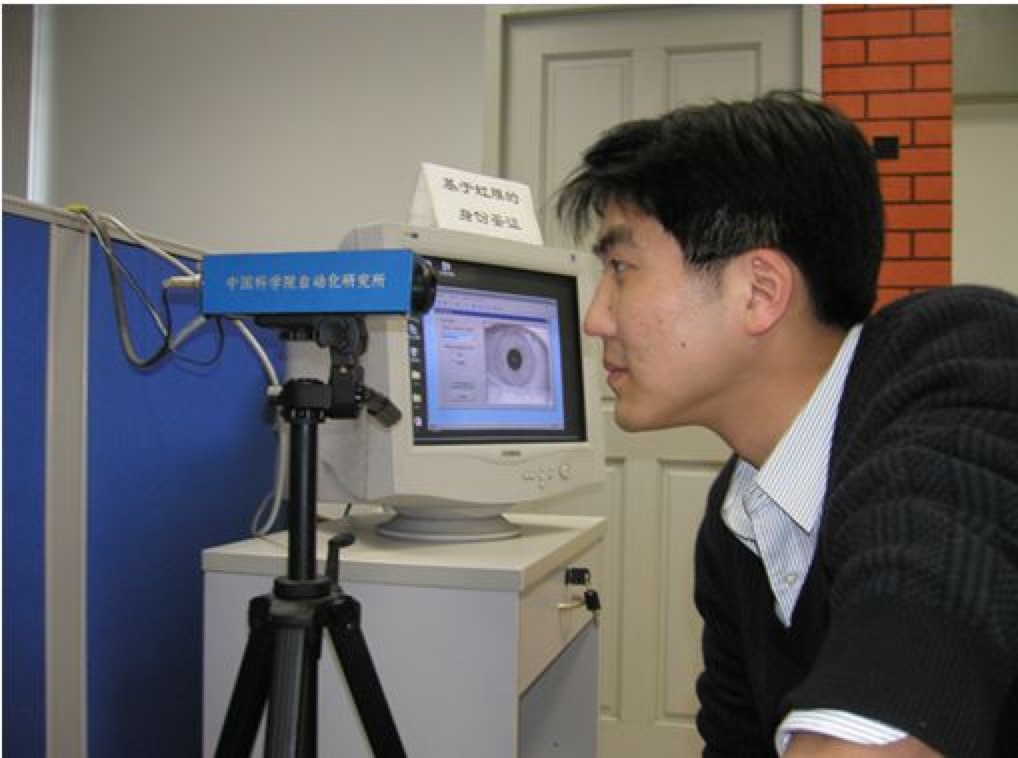
\includegraphics[width=6cm]{device.jpg}
	\end{textblock*}	

\end{frame}

%------------------------------------------------

\begin{frame}
	\frametitle{研究背景}
	\begin{varblock}[0.5\textwidth]{}
		虹膜识别的瓶颈问题之一是难以收集到高质量的虹膜图像。虹膜图像通常伴随以下三种退化:
		\begin{itemize}
			\item 在远距离场景下,采集到的虹膜图像\alert{分辨率太低}。
			\item 如果受试者站在相机的景深之外,会产生\alert{离焦模糊}。
			\item 在采集过程中,如果受试者在移动,会造成\alert{运动模糊}。 
		\end{itemize}
	\end{varblock}	

	\begin{textblock*}{7cm}(8.6cm,2cm) % {block width} (coords)
		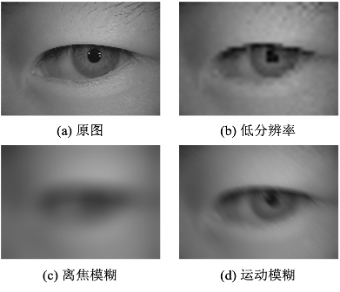
\includegraphics[width=7cm]{degraded.png}
	\end{textblock*}	

\end{frame}


%------------------------------------------------

\section{研究内容}

\subsection{基于深度级注意力机制的虹膜图像修复方法}

\subsubsection{理论分析}

%------------------------------------------------

\begin{frame}
	\frametitle{\large 基于深度级注意力机制的虹膜图像修复方法}
	\framesubtitle{\normalsize 骨干网络} % Optional subtitle
	\begin{varblock}[0.7\textwidth]{}
		现有的方法一般运用了卷积神经网络,只能利用局部信息,无法利用全局信息,导致特征提取能力较弱,无法精确地修复虹膜图像。
	\end{varblock}	
	\begin{varblock}[0.7\textwidth]{}
		本章提出了基于深度级注意力机制的虹膜图像修复方法,可以对长距离的像素依赖进行建模,并且能在推理过程中,根据输入来动态地调整参数,同时,实现了线性的计算复杂度,使得本章方法的计算量小于现有的基于注意力机制的方法。
	\end{varblock}	
	\begin{textblock*}{4.5cm}(11.3cm,1.8cm) % {block width} (coords)
		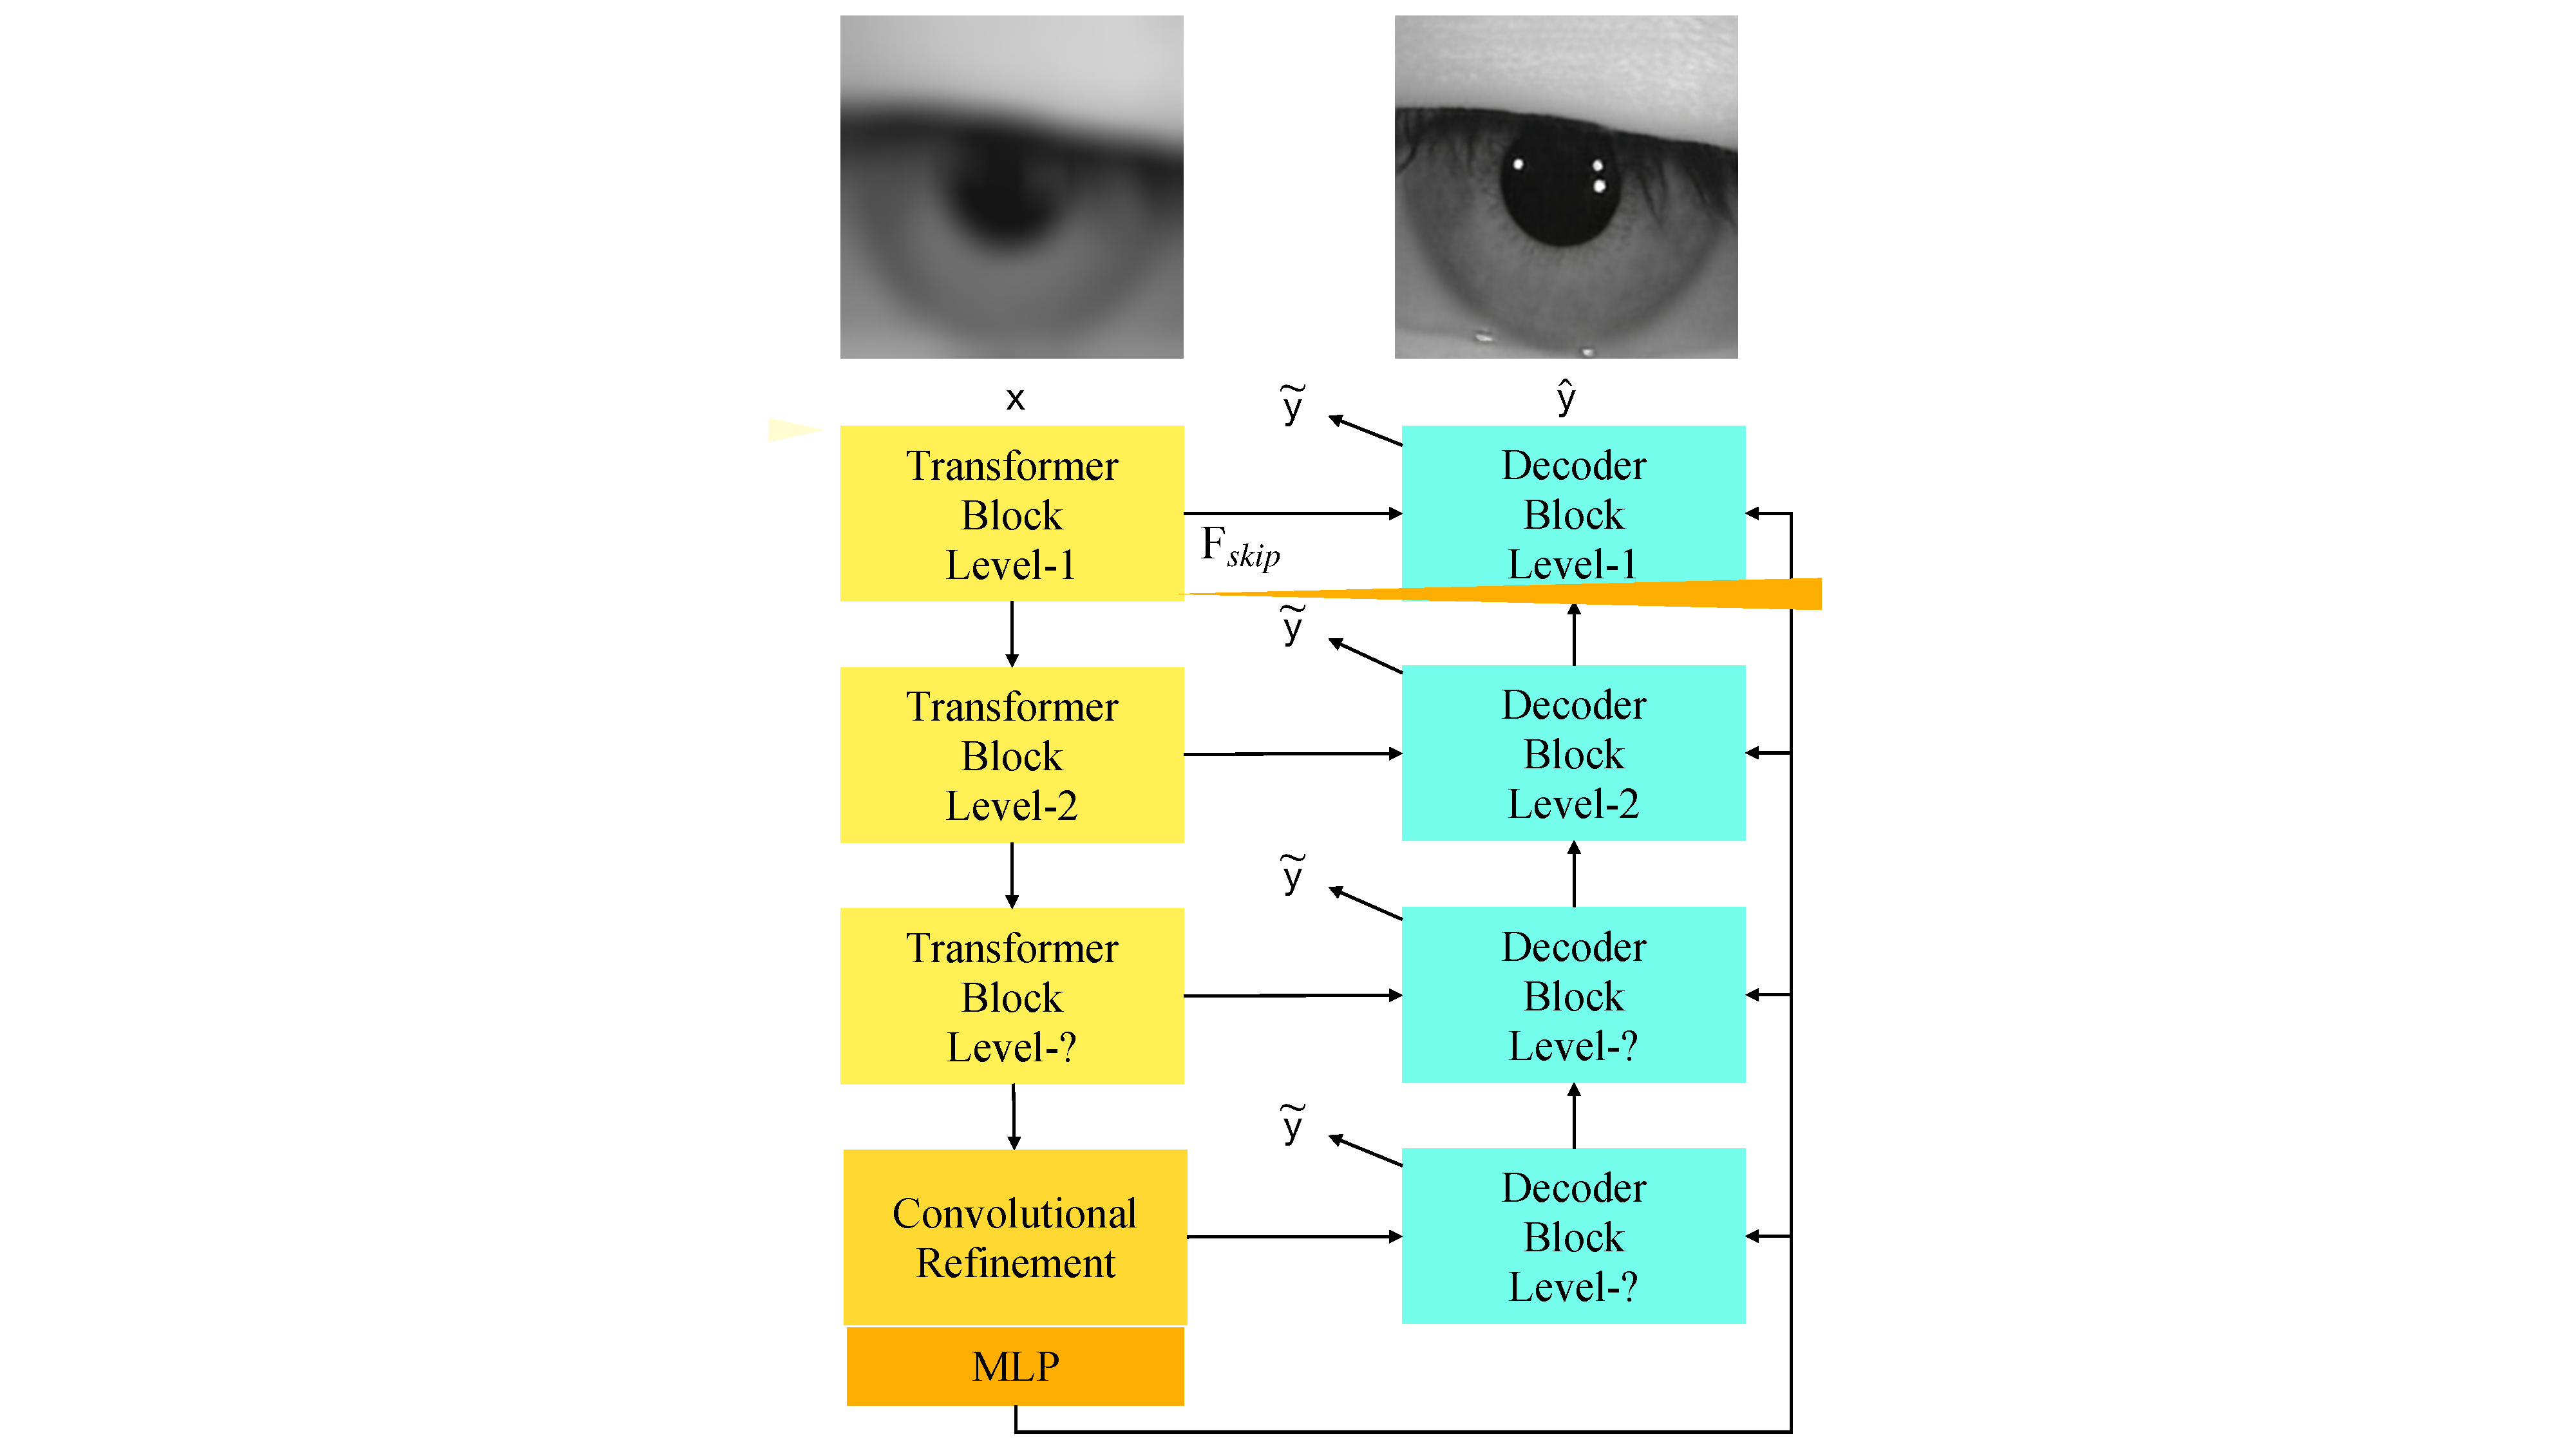
\includegraphics[width=4.5cm]{chanel1.pdf}
	\end{textblock*}		

\end{frame}

%------------------------------------------------

\begin{frame}
	\frametitle{\large 基于深度级注意力机制的虹膜图像修复方法}
	\framesubtitle{\normalsize 深度级注意力机制} % Optional subtitle
	\begin{varblock}[0.8\textwidth]{}
		\small 在传统的自注意力机制中,注意力分数$\alpha=\textbf{Q}\cdot\textbf{K}$的时间和空间复杂度为 $\mathcal{O}(\textit{W}^{2}\textit{H}^{2})$。因此,将这样的自注意力机制用到图像修复任务中,会产生过大的计算开销。
	\end{varblock}	
	\begin{varblock}[0.8\textwidth]{}
		\small 为了缓解这个问题,本章提出了具有线性复杂度的深度级注意力机制。
		\begin{enumerate}
			\setlength\itemsep{0.1ex}
			\item 使用像素卷积,收集一个像素在所有的通道范围内的内容信息,这个结构可以进一步提取通道范围内的特征。
			\item 使用深度卷积,提取一个通道中,所有空间范围内的内容信息。
		\end{enumerate}		
	\end{varblock}	
	\begin{textblock*}{2.4cm}(13.1cm,1.6cm) % {block width} (coords)
		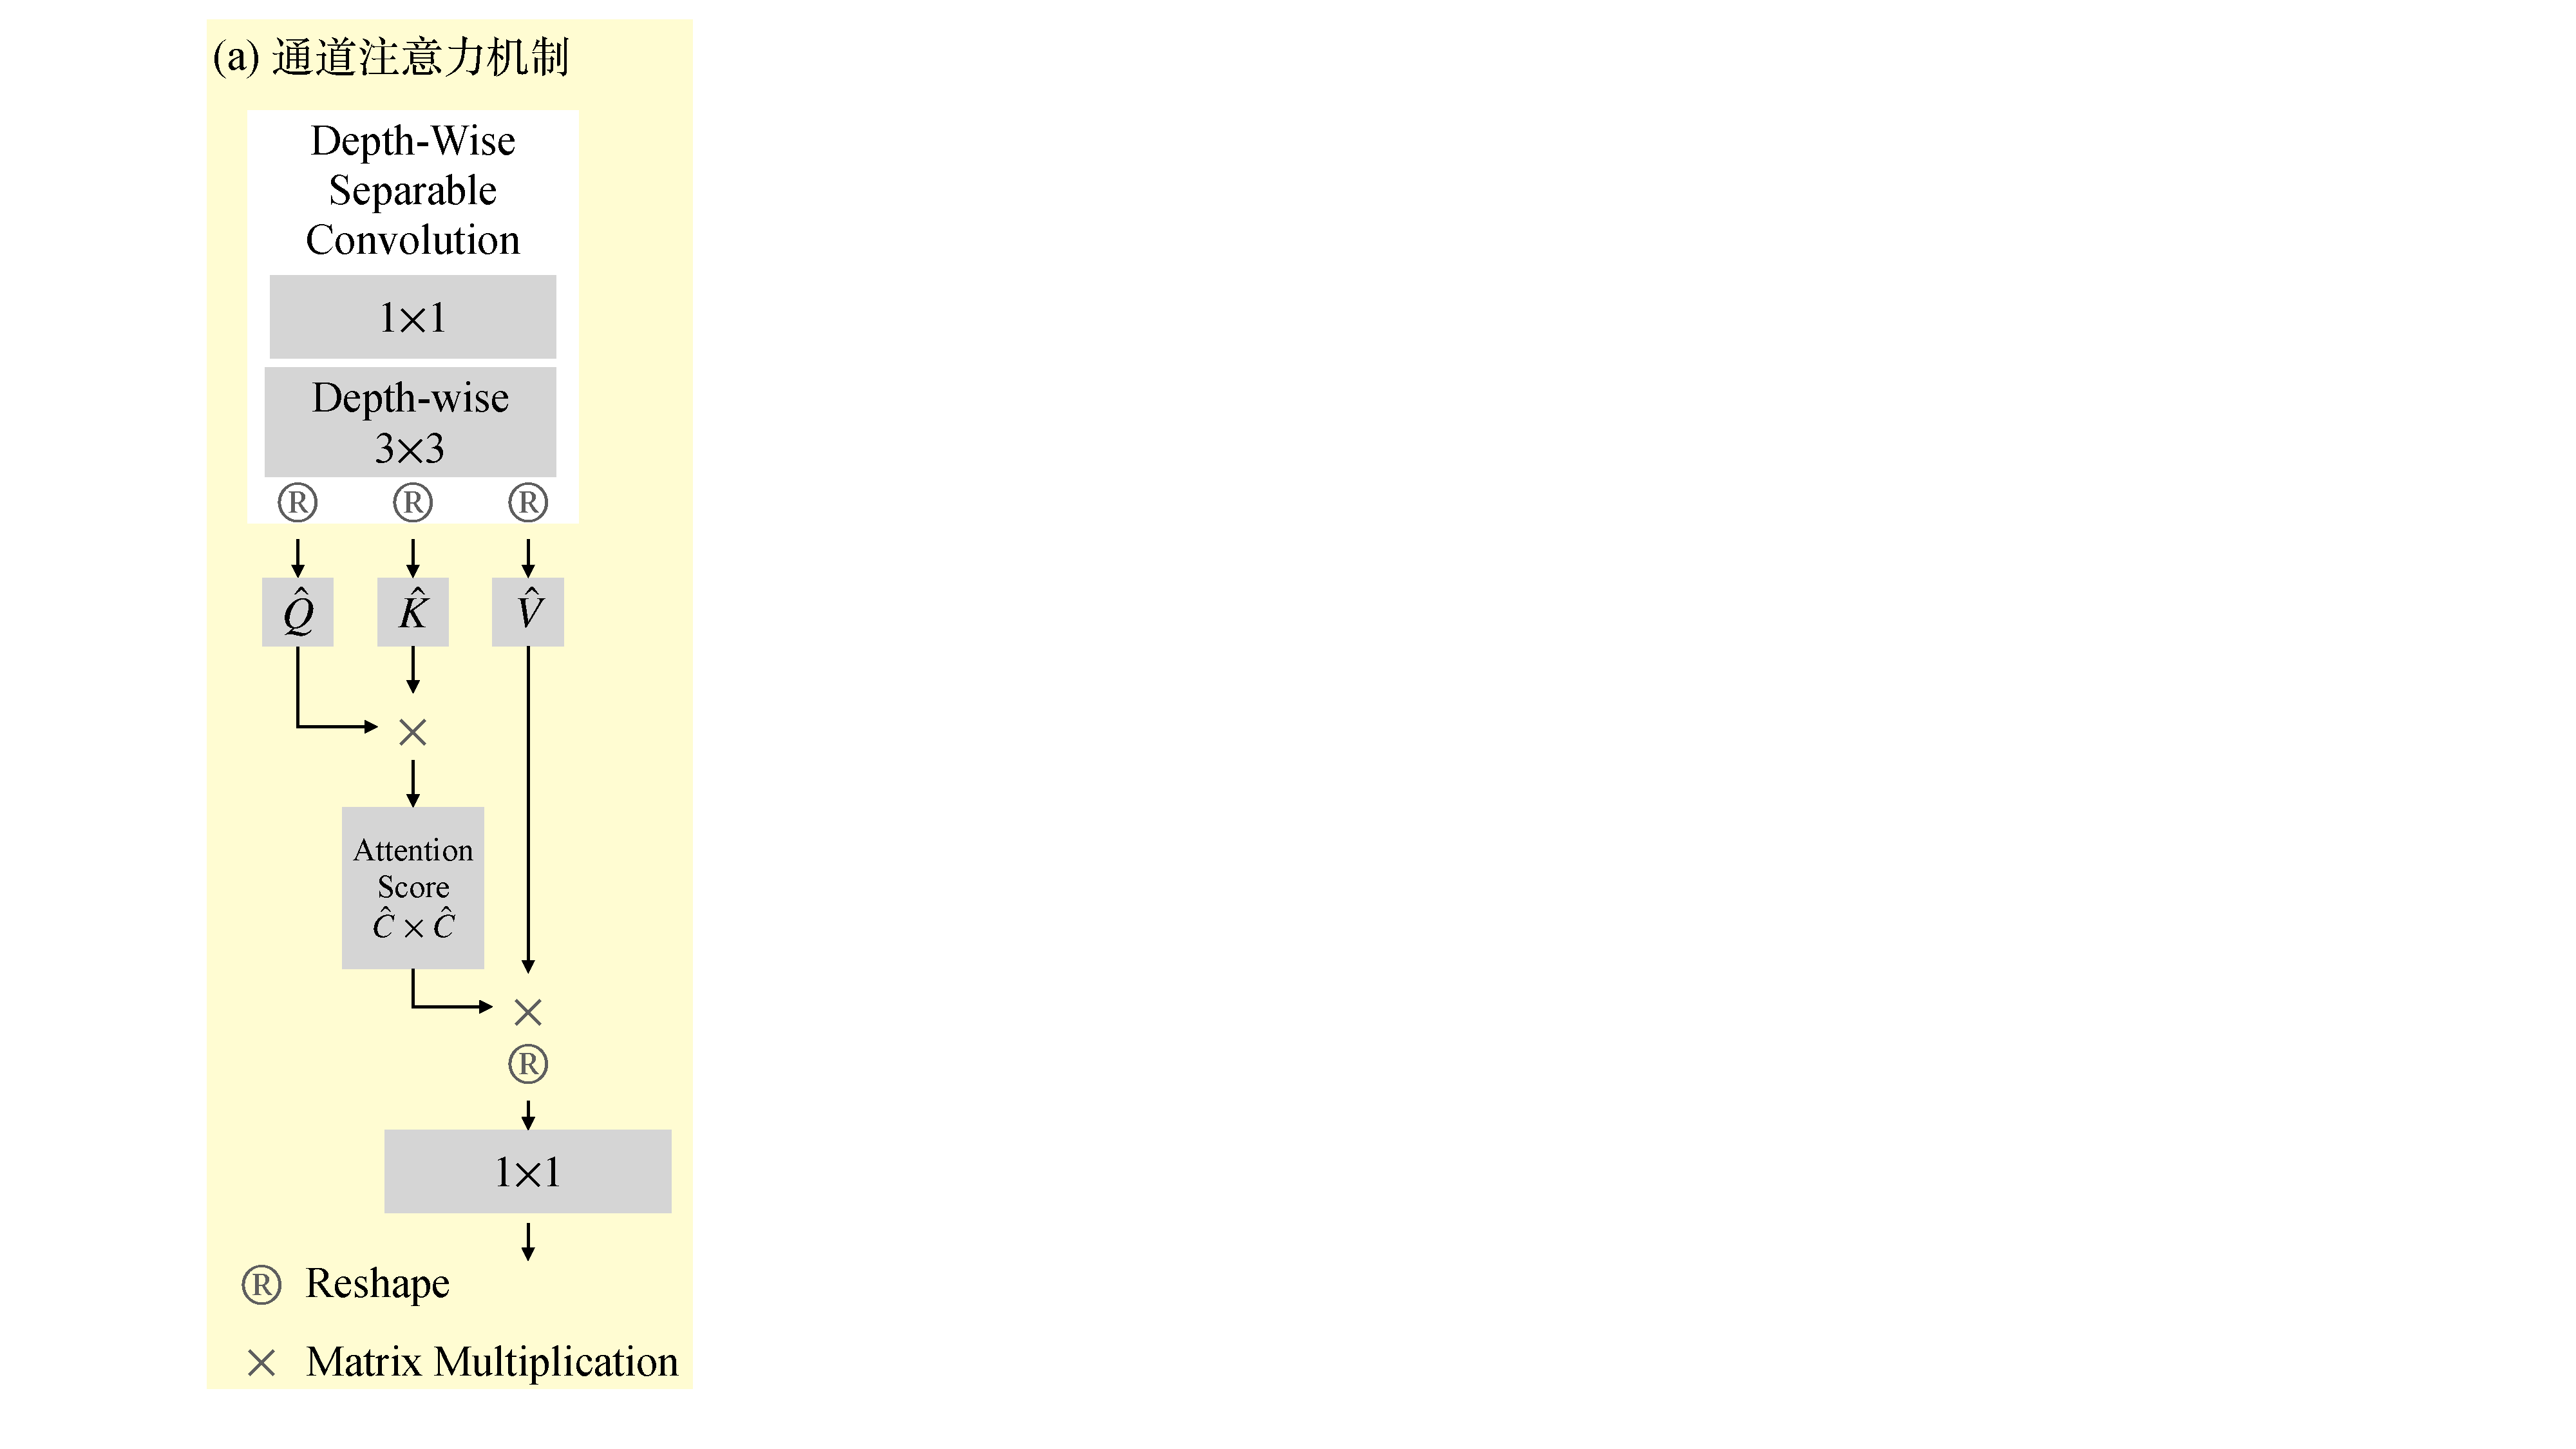
\includegraphics[width=2.4cm]{chanel2.pdf}
	\end{textblock*}		

\end{frame}

%------------------------------------------------

\begin{frame}
	\frametitle{\large 基于深度级注意力机制的虹膜图像修复方法}
	\framesubtitle{\normalsize 深度级激活网络} % Optional subtitle
	\begin{varblock}[0.8\textwidth]{}
		\small 传统的激活网络以完全相同的方法独立地处理每个像素上的信息。
	\end{varblock}	
	\begin{varblock}[0.8\textwidth]{}
		\small 本章采用了深度级激活网络。该网络中的两个机制,对提升表征学习能力有所帮助:
		\begin{enumerate}
			\setlength\itemsep{0.1ex}
			\item 门控机制:输入并行经过两条线性变换路径,其中一条路径添加了GELU非线性激活函数,然后将这两条路径做数量积。
			\item 深度级卷积:保持了从相邻像素编码信息的能力,此外,可以有效地学习到图像局部的结构。
		\end{enumerate}		
	\end{varblock}	
	\begin{textblock*}{2.4cm}(13cm,1.6cm) % {block width} (coords)
		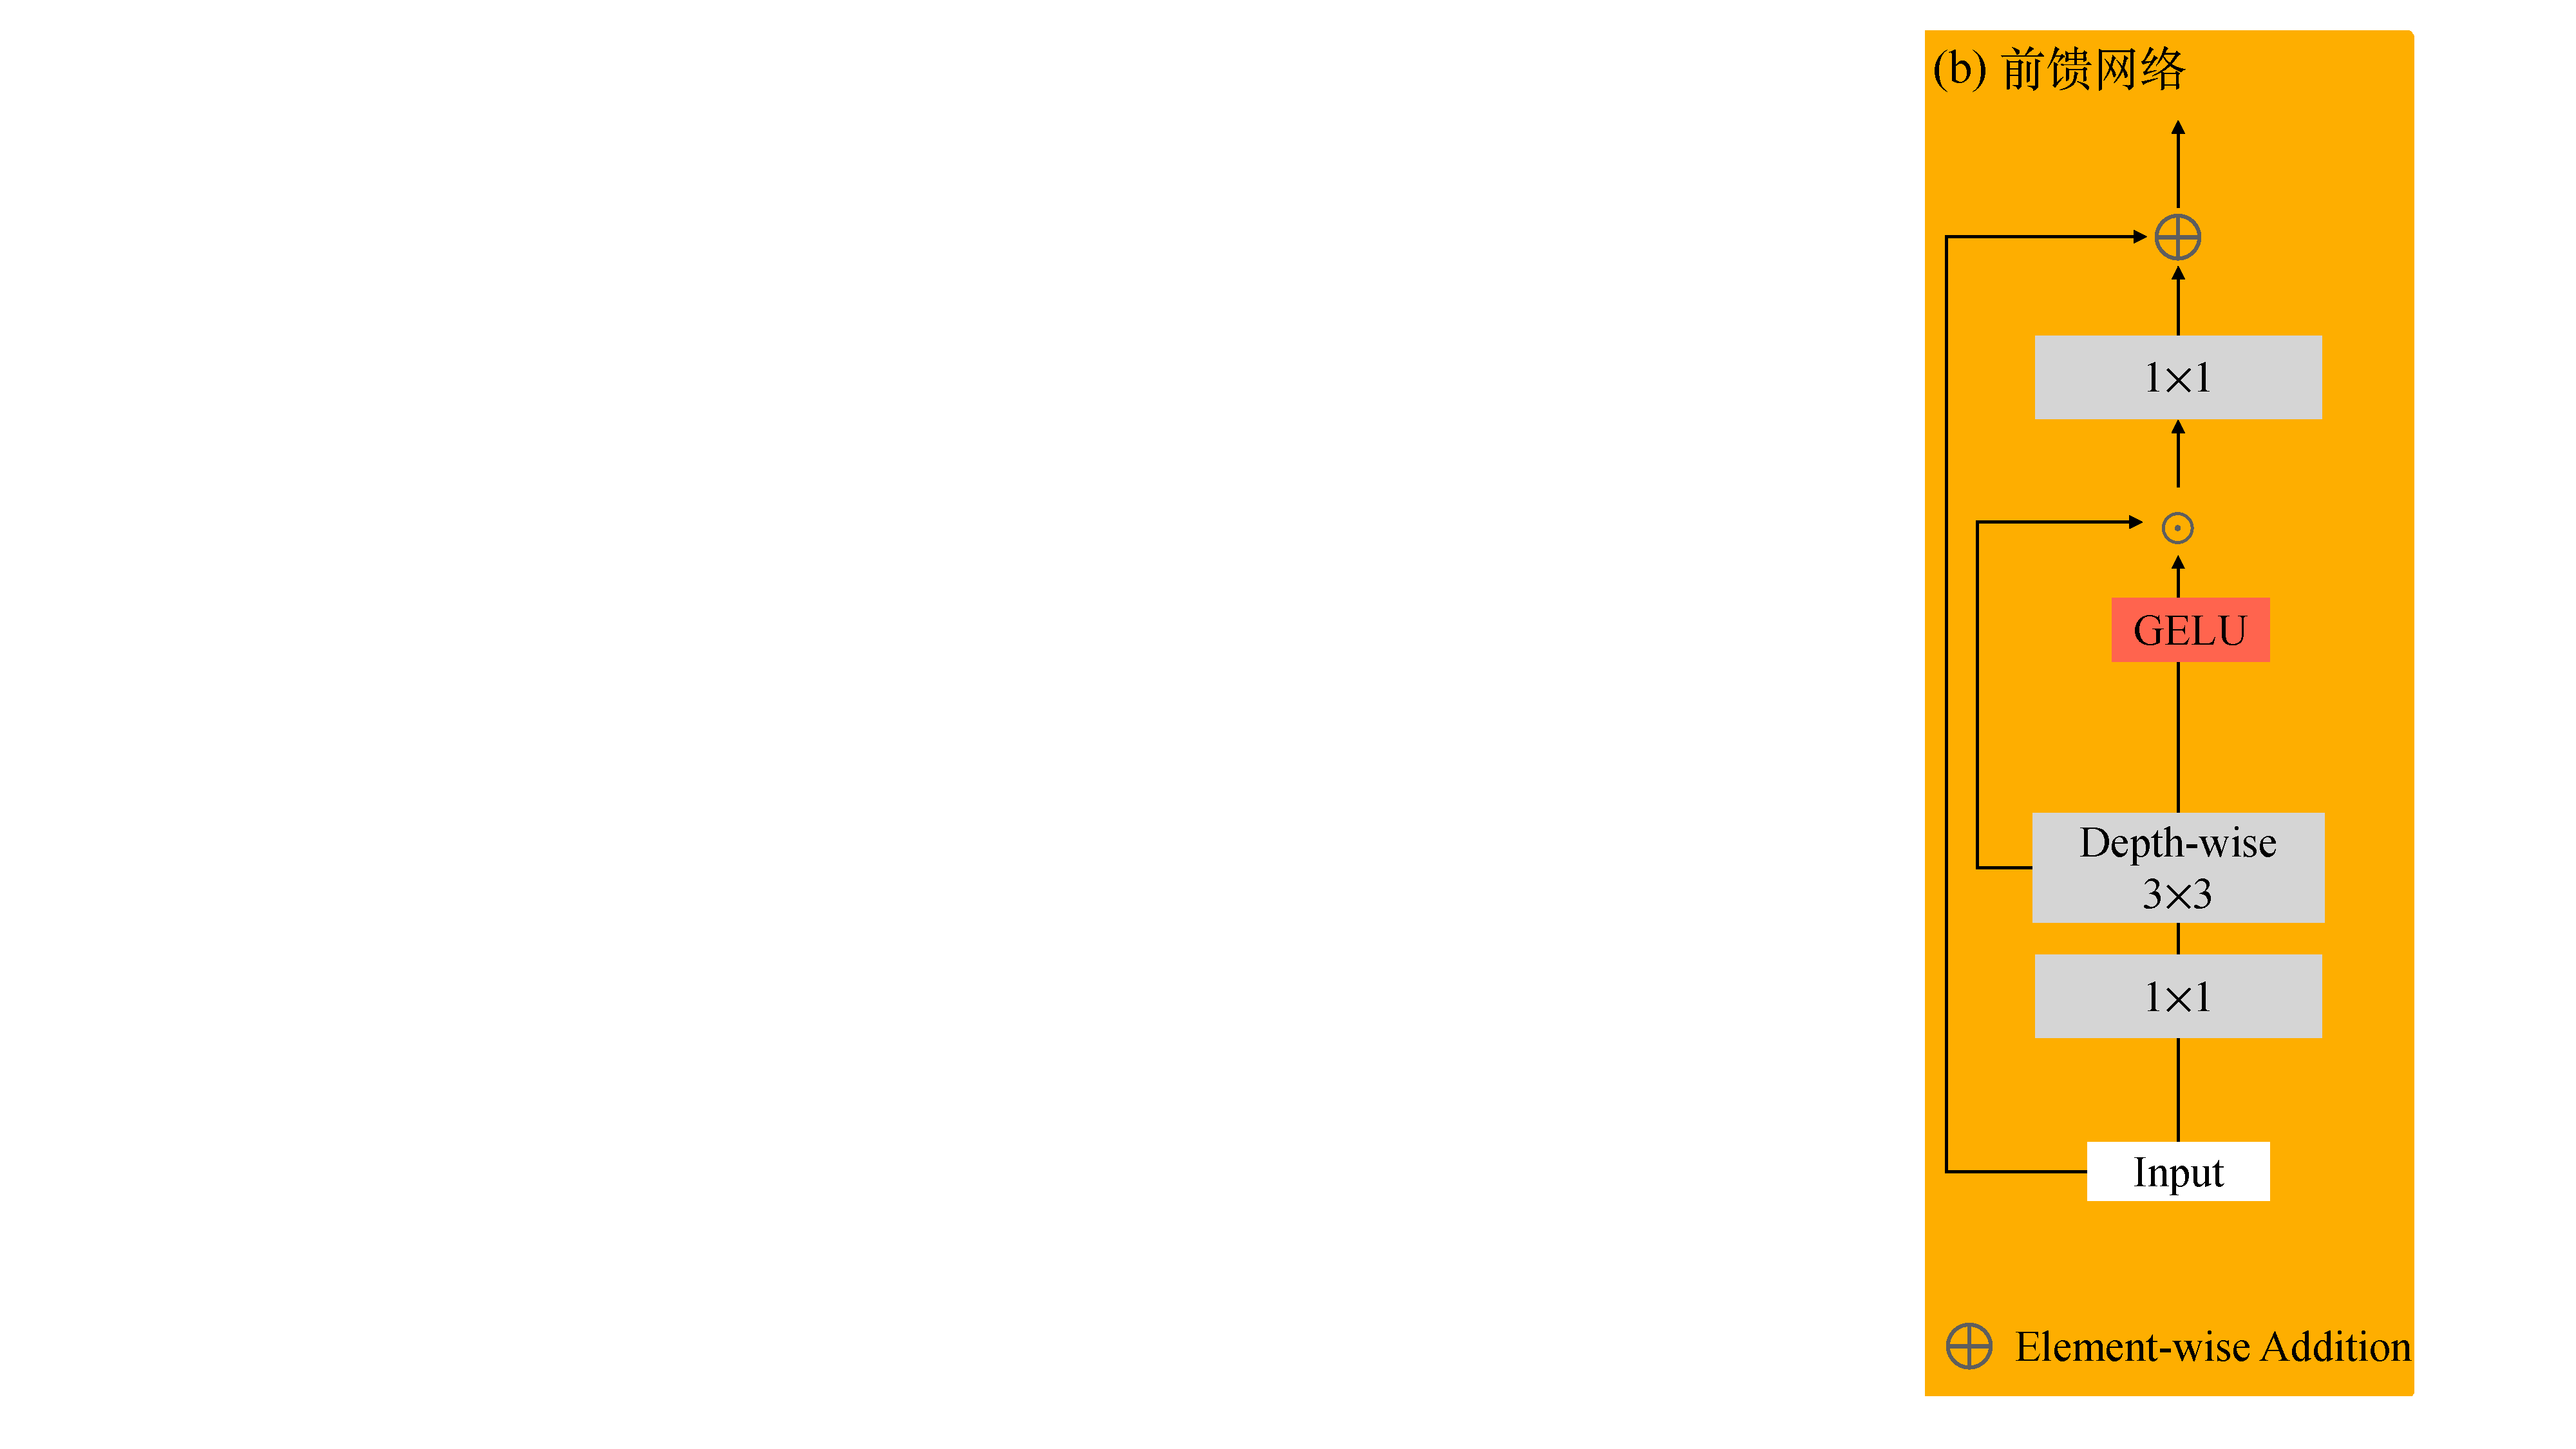
\includegraphics[width=2.4cm]{chanel3.pdf}
	\end{textblock*}		

\end{frame}

%------------------------------------------------

\subsubsection{实验配置与结果}

\begin{frame}
	\frametitle{实验数据}
	\framesubtitle{} % Optional subtitle
	\begin{varblock}[0.55\textwidth]{}
		\small 本文使用了中科院虹膜数据集CASIA-IrisV4中的
		\begin{enumerate}
			\item 灯光数据集CASIA-Iris-Lamp,包含来自411个受试者的16,212张虹膜图像,共822个类别。类内变化的主要来源是瞳孔的收缩。
			\item 千人数据集CASIA-Iris-Thousand,包含来自1,000个受试者的 20,000张虹膜图像,共2,000个类别。类内变化的主要来源是眼镜的镜面反射。
		\end{enumerate}			
	\end{varblock}	

	\begin{textblock*}{6cm}(9.5cm,2.2cm) % {block width} (coords)
		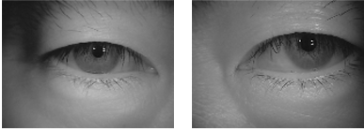
\includegraphics[width=6cm]{lamp.png}
	\end{textblock*}	
	\begin{textblock*}{6cm}(9.5cm,5.4cm) % {block width} (coords)
		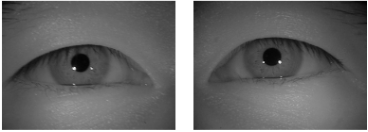
\includegraphics[width=6cm]{thousand.png}
	\end{textblock*}	
\end{frame}

%------------------------------------------------

\begin{frame}
	\frametitle{实验数据}
	\framesubtitle{} % Optional subtitle
	\begin{varblock}[0.6\textwidth]{}
		\small 
		\begin{itemize}
			\item 本文先将上述两数据集进行合并,删除虹膜处有遮挡的数据,得到28,089张虹膜图像,其中包含2,738个类别,用于本文的实验。
			\item 接着用虹膜检测算法定位虹膜,然后进行裁剪,分辨率由640$\times$480变为224$\times$224。
			\item 最后将图像通过随机的高斯模糊核、运动模糊核和下采样因子进行退化,用来模拟真实世界中图像的退化。
			\item 测试集与训练集的合成方式相同。并且,二者没有重叠。
		\end{itemize}	
	\end{varblock}	

	\begin{textblock*}{5.5cm}(10cm,2cm) % {block width} (coords)
		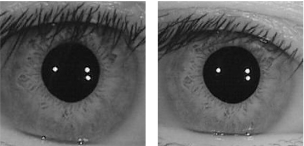
\includegraphics[width=5.5cm]{mixing.png}
	\end{textblock*}	
	\begin{textblock*}{1.4cm}(10.6cm,5.5cm) % {block width} (coords)
		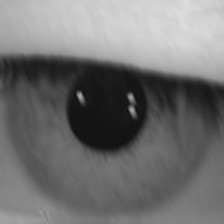
\includegraphics[width=1.4cm]{cubic1.png}
	\end{textblock*}		
	\begin{textblock*}{2.2cm}(13.1cm,5cm) % {block width} (coords)
		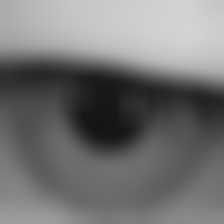
\includegraphics[width=2.2cm]{cubic2.png}
	\end{textblock*}	
\end{frame}

%------------------------------------------------

\begin{frame}
	\frametitle{\large 基于深度级注意力机制的虹膜图像修复方法}
	\framesubtitle{\normalsize 实验设置} % Optional subtitle
	\begin{varblock}[0.65\textwidth]{}
		\begin{itemize}
			\item Transformer模块的层级数为4,每个层级包含1个Transformer块。从层级1到层级4,注意力机制“头”的数目分别为[1, 2, 4, 8]。
			\item 由浅到深每个层级输出图像分辨率分别为$[256^2, 128^2, 64^2, 32^2, 16^2, 8^2, 4^2]$。
			\item Adam优化器,学习率设为$2 \times 10^{-4}$。
			\item 深度学习框架为PyTorch。
			\item GPU型号为NVIDIA Tesla v100。
		\end{itemize}	
	\end{varblock}	

	\begin{textblock*}{5.5cm}(10.5cm,2cm) % {block width} (coords)
		
\includegraphics[width=5.5cm]{pytorch.jpg}
	\end{textblock*}	
	\begin{textblock*}{4cm}(11cm,4cm) % {block width} (coords)
		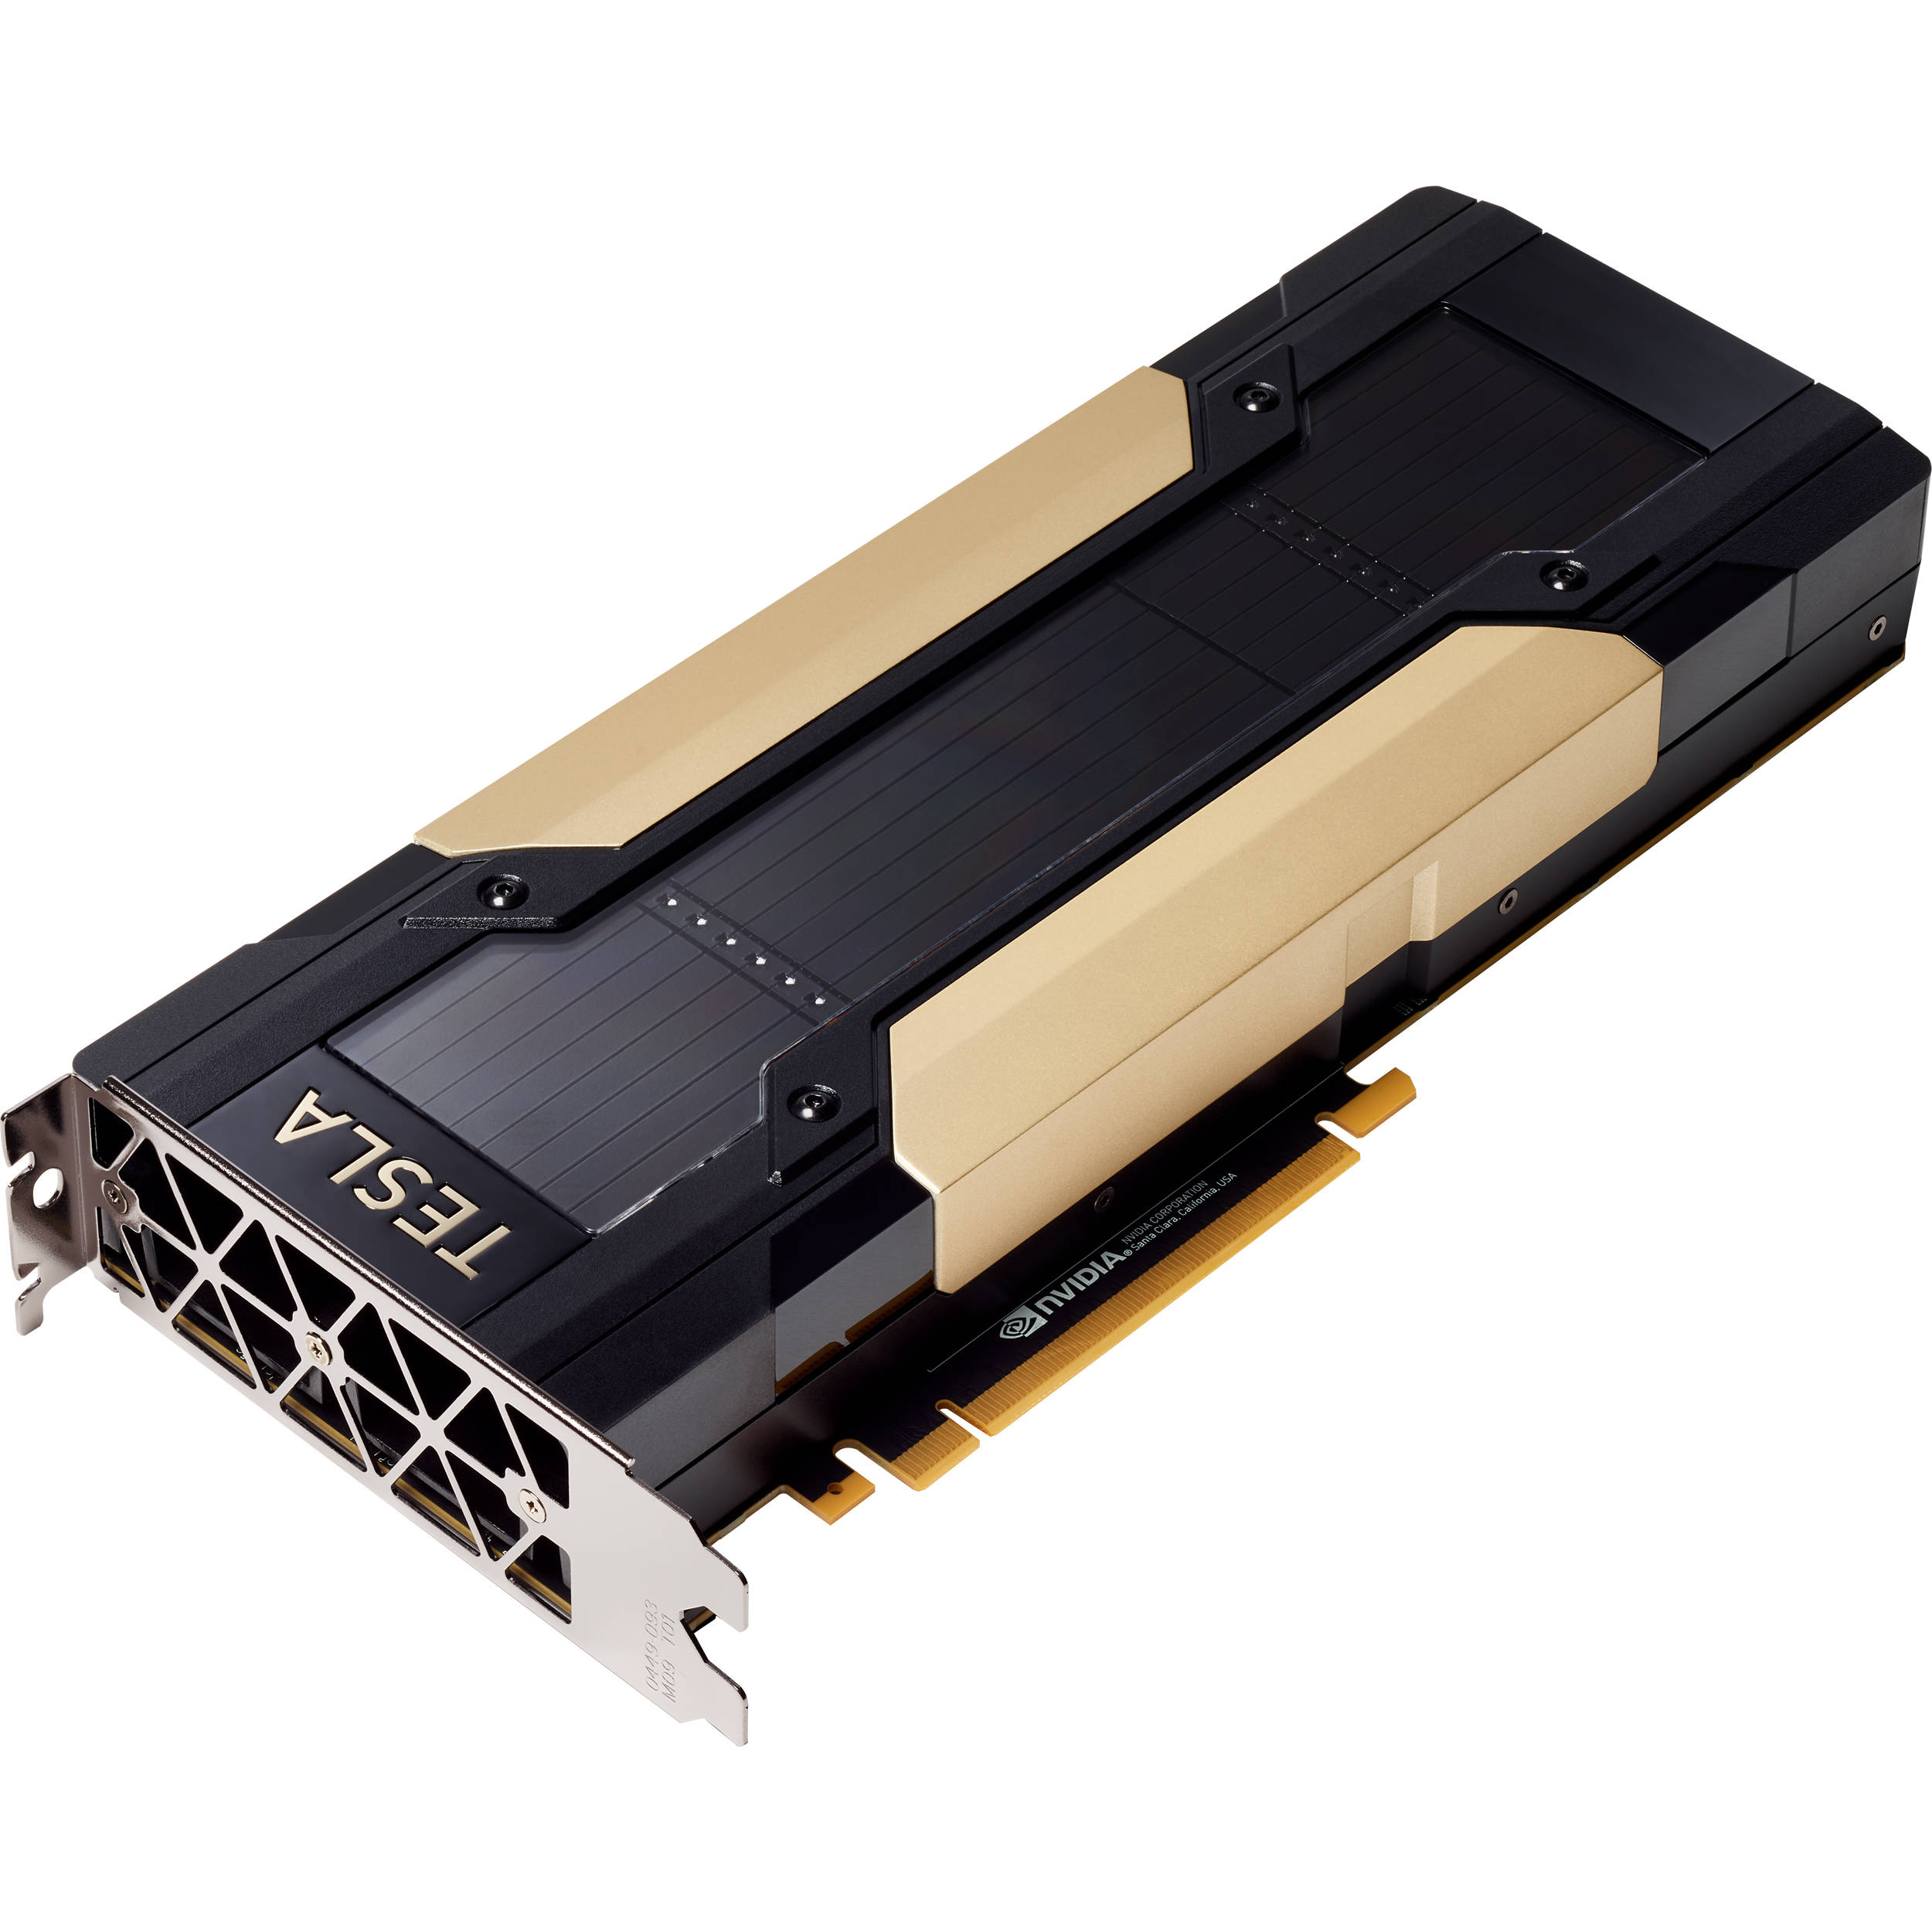
\includegraphics[width=4cm]{v100.jpg}
	\end{textblock*}		

\end{frame}

%------------------------------------------------

\begin{frame}
	\frametitle{定量实验结果}
	\framesubtitle{} % Optional subtitle
	
	\begin{table}
	\footnotesize
\begin{tabular}{ccc ccc ccc}
  \hline
  % after \\: \hline or \cline{col1-col2} \cline{col3-col4} ...
Method & AUC $\uparrow$ & EER $\downarrow$	& \makecell{TAR@FAR \\ =0.001 $\uparrow$} & \makecell{TAR@FAR \\ =0.01 $\uparrow$} & PSNR $\uparrow$ & SSIM $\uparrow$ & LPIPS $\downarrow$ \\ \hline
输入 & 0.9521 & 0.1153 & 0.1992 & 0.5361 & 30.68 & 0.8336 & 0.2865 \\
EDSR & 0.9796 & 0.0705 & 0.5356 & 0.7538 & \textbf{34.15} & \textbf{0.8808} & 0.1249 \\
RCAN & 0.9818 & 0.0679 & 0.5608 & 0.7666 & 33.57 & 0.8789 & 0.1324 \\
SRGAN & 0.9732 & 0.0853	& 0.3960 & 0.6705 & 32.85 & 0.8695 & 0.1311 \\
ESRGAN & 0.9585	& 0.1093 & 0.4816 & 0.6876 & 30.29 & 0.8314 & \textbf{0.1189} \\
SISN & 0.9836 & 0.0542 & 0.5878 & 0.8274 & 32.36 & 0.8729 & 0.1350 \\
\alert{本章方法} & \alert{0.9864} & \alert{0.0532} & \alert{0.7475} & \alert{0.8773} & 32.82 & 0.8754 & 0.1513 \\
 \hline
原始图像 & 0.9914 & 0.0274 & 0.9323& 0.9613 & - & - & -\\ \hline
\end{tabular}
		\caption{基于深度级注意力机制的虹膜图像修复方法与现有方法的定量结果对比。}
	\end{table}
\end{frame}

%------------------------------------------------

\begin{frame}
	\frametitle{定性实验结果}
	
	\begin{figure}
\centering
\begin{minipage}[t]{0.11\textwidth}
\centering

\includegraphics[width=1\linewidth]{cubic3.png}
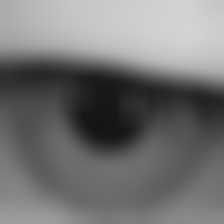
\includegraphics[width=1\linewidth]{cubic2.png}
\centerline{\footnotesize 输入}\medskip
\end{minipage}
\begin{minipage}[t]{0.11\textwidth}
\centering
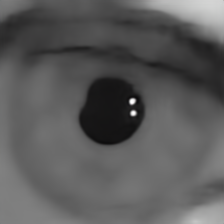
\includegraphics[width=1\linewidth]{edsr3.png}
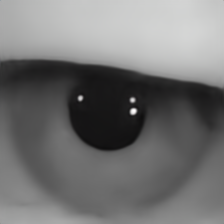
\includegraphics[width=1\linewidth]{edsr2.png}
\centerline{\footnotesize EDSR}\medskip
\end{minipage}
\begin{minipage}[t]{0.11\textwidth}
\centering
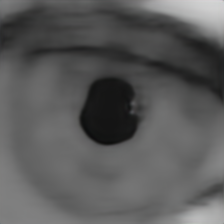
\includegraphics[width=1\linewidth]{rcan3.png}
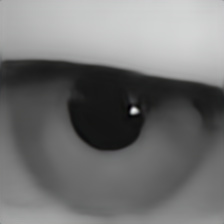
\includegraphics[width=1\linewidth]{rcan2.png}
\centerline{\footnotesize RCAN}\medskip
\end{minipage}
\begin{minipage}[t]{0.11\textwidth}
\centering
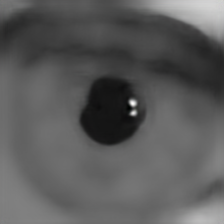
\includegraphics[width=1\linewidth]{srgan3.png}
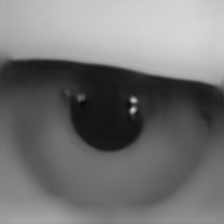
\includegraphics[width=1\linewidth]{srgan2.png}
\centerline{\footnotesize SRGAN}\medskip
\end{minipage}
\begin{minipage}[t]{0.11\textwidth}
\centering
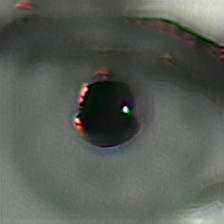
\includegraphics[width=1\linewidth]{esrgan3.png}
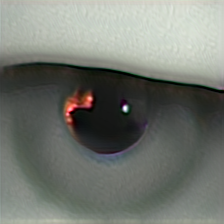
\includegraphics[width=1\linewidth]{esrgan2.png}
\centerline{\footnotesize ESRGAN}\medskip
\end{minipage}
\begin{minipage}[t]{0.11\textwidth}
\centering
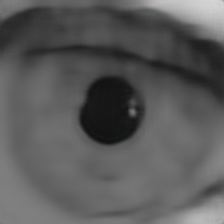
\includegraphics[width=1\linewidth]{sisn_S2309L07_HR.png}
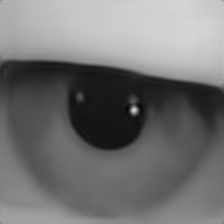
\includegraphics[width=1\linewidth]{sisn_S2308L02_HR.png}
\centerline{\footnotesize SISN}\medskip
\end{minipage}
\begin{minipage}[t]{0.11\textwidth}
\centering
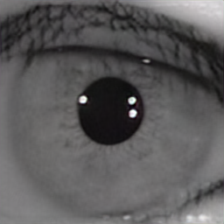
\includegraphics[width=1\linewidth]{S2309L07_withoutprior.png}
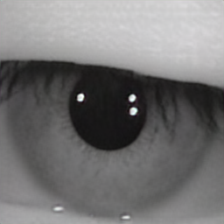
\includegraphics[width=1\linewidth]{S2308L02_withoutprior.png}
\centerline{\footnotesize \alert{本章方法}}\medskip
\end{minipage}
\begin{minipage}[t]{0.11\textwidth}
\centering
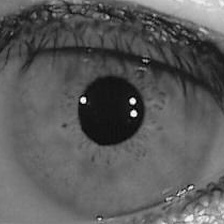
\includegraphics[width=1\linewidth]{gt3.png}
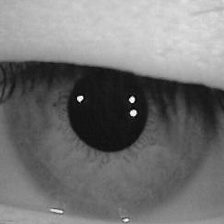
\includegraphics[width=1\linewidth]{gt2.png}
\centerline{\footnotesize 原始图像}\medskip
\end{minipage}
\caption{基于深度级注意力机制的虹膜图像修复方法与现有方法的定性实验结果对比。}
	\end{figure}
\end{frame}

%------------------------------------------------

\begin{frame}
	\frametitle{虹膜识别性能测试}
	\begin{figure}
\centering
% \centerline{\epsfig{figure=image1.ps,width=8.5cm}}
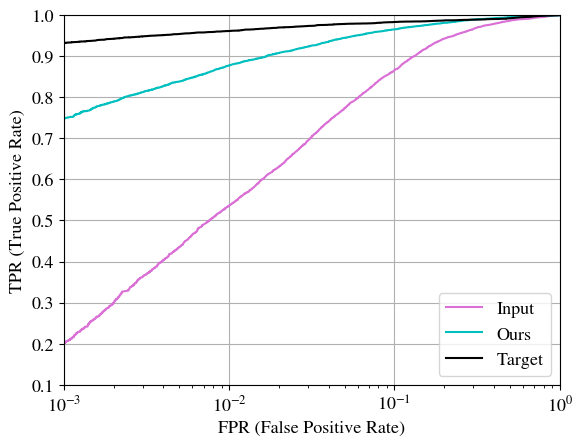
\includegraphics[width=0.5\textwidth]{roc_without_prior.png}
\caption{基于深度级注意力机制的虹膜图像修复方法的ROC曲线。}
	\end{figure}
\end{frame}

%------------------------------------------------

\begin{frame}
	\frametitle{消融实验}
	\framesubtitle{} % Optional subtitle
	
	\begin{table}
	\footnotesize
\begin{tabular}{ccc ccc ccc}
  \hline
  % after \\: \hline or \cline{col1-col2} \cline{col3-col4} ...
Method & AUC $\uparrow$ & EER $\downarrow$	& \makecell{TAR@FAR \\ =0.001 $\uparrow$} & \makecell{TAR@FAR \\ =0.01 $\uparrow$} & PSNR $\uparrow$ & SSIM $\uparrow$ \\ \hline
w/o Transformer & 0.9523 & 0.1251 & 0.5342 & 0.6753 & 30.01 & 0.8072 \\
w/o Pyramid Loss & 0.9905 & 0.0456 & 0.7908 & 0.9033  & 33.42 & 0.8791 \\
w/o Perceptual Loss & 0.9521 & 0.1252 & 0.5266 & 0.6725 & 29.50 & 0.8068 \\
w/o Adversarial Loss & 0.9864 & 0.0532 & 0.7200 & 0.8702 & 32.12 & 0.8629 \\
本章方法 & 0.9864 & 0.0532 & 0.7475 & 0.8773 & 32.82 & 0.8754 \\
 \hline
\end{tabular}
		\caption{基于深度级注意力机制的虹膜图像修复方法的消融实验结果。}
	\end{table}
\end{frame}

%------------------------------------------------

\subsection{基于生成式先验知识的虹膜图像修复方法}

\subsubsection{理论分析}

\begin{frame}
	\frametitle{\large 基于生成式先验知识的虹膜图像修复方法}
	\framesubtitle{\normalsize 骨干网络} % Optional subtitle
	\begin{varblock}[0.7\textwidth]{}
		\small 生成对抗网络一般用于直接生成目标图像。由于虹膜具有复杂的微结构,借助先验知识有助于修复得到更加逼真的纹理细节。
	\end{varblock}	
	\begin{varblock}[0.7\textwidth]{}
		\small 虹膜生成式先验知识是一个预训练好的虹膜生成对抗网络,它捕获了虹膜的特征分布,储存到了网络的参数中。本章利用虹膜生成式先验知识,指导图像修复工作。
	\end{varblock}	
	\begin{varblock}[0.7\textwidth]{}
		\small 解码器为StyleGANv2的生成器,包含了多层级的生成器块,生成器块的数目由输入图像的分辨率决定。
	\end{varblock}		
	\begin{textblock*}{4.5cm}(11.2cm,1.8cm) % {block width} (coords)
		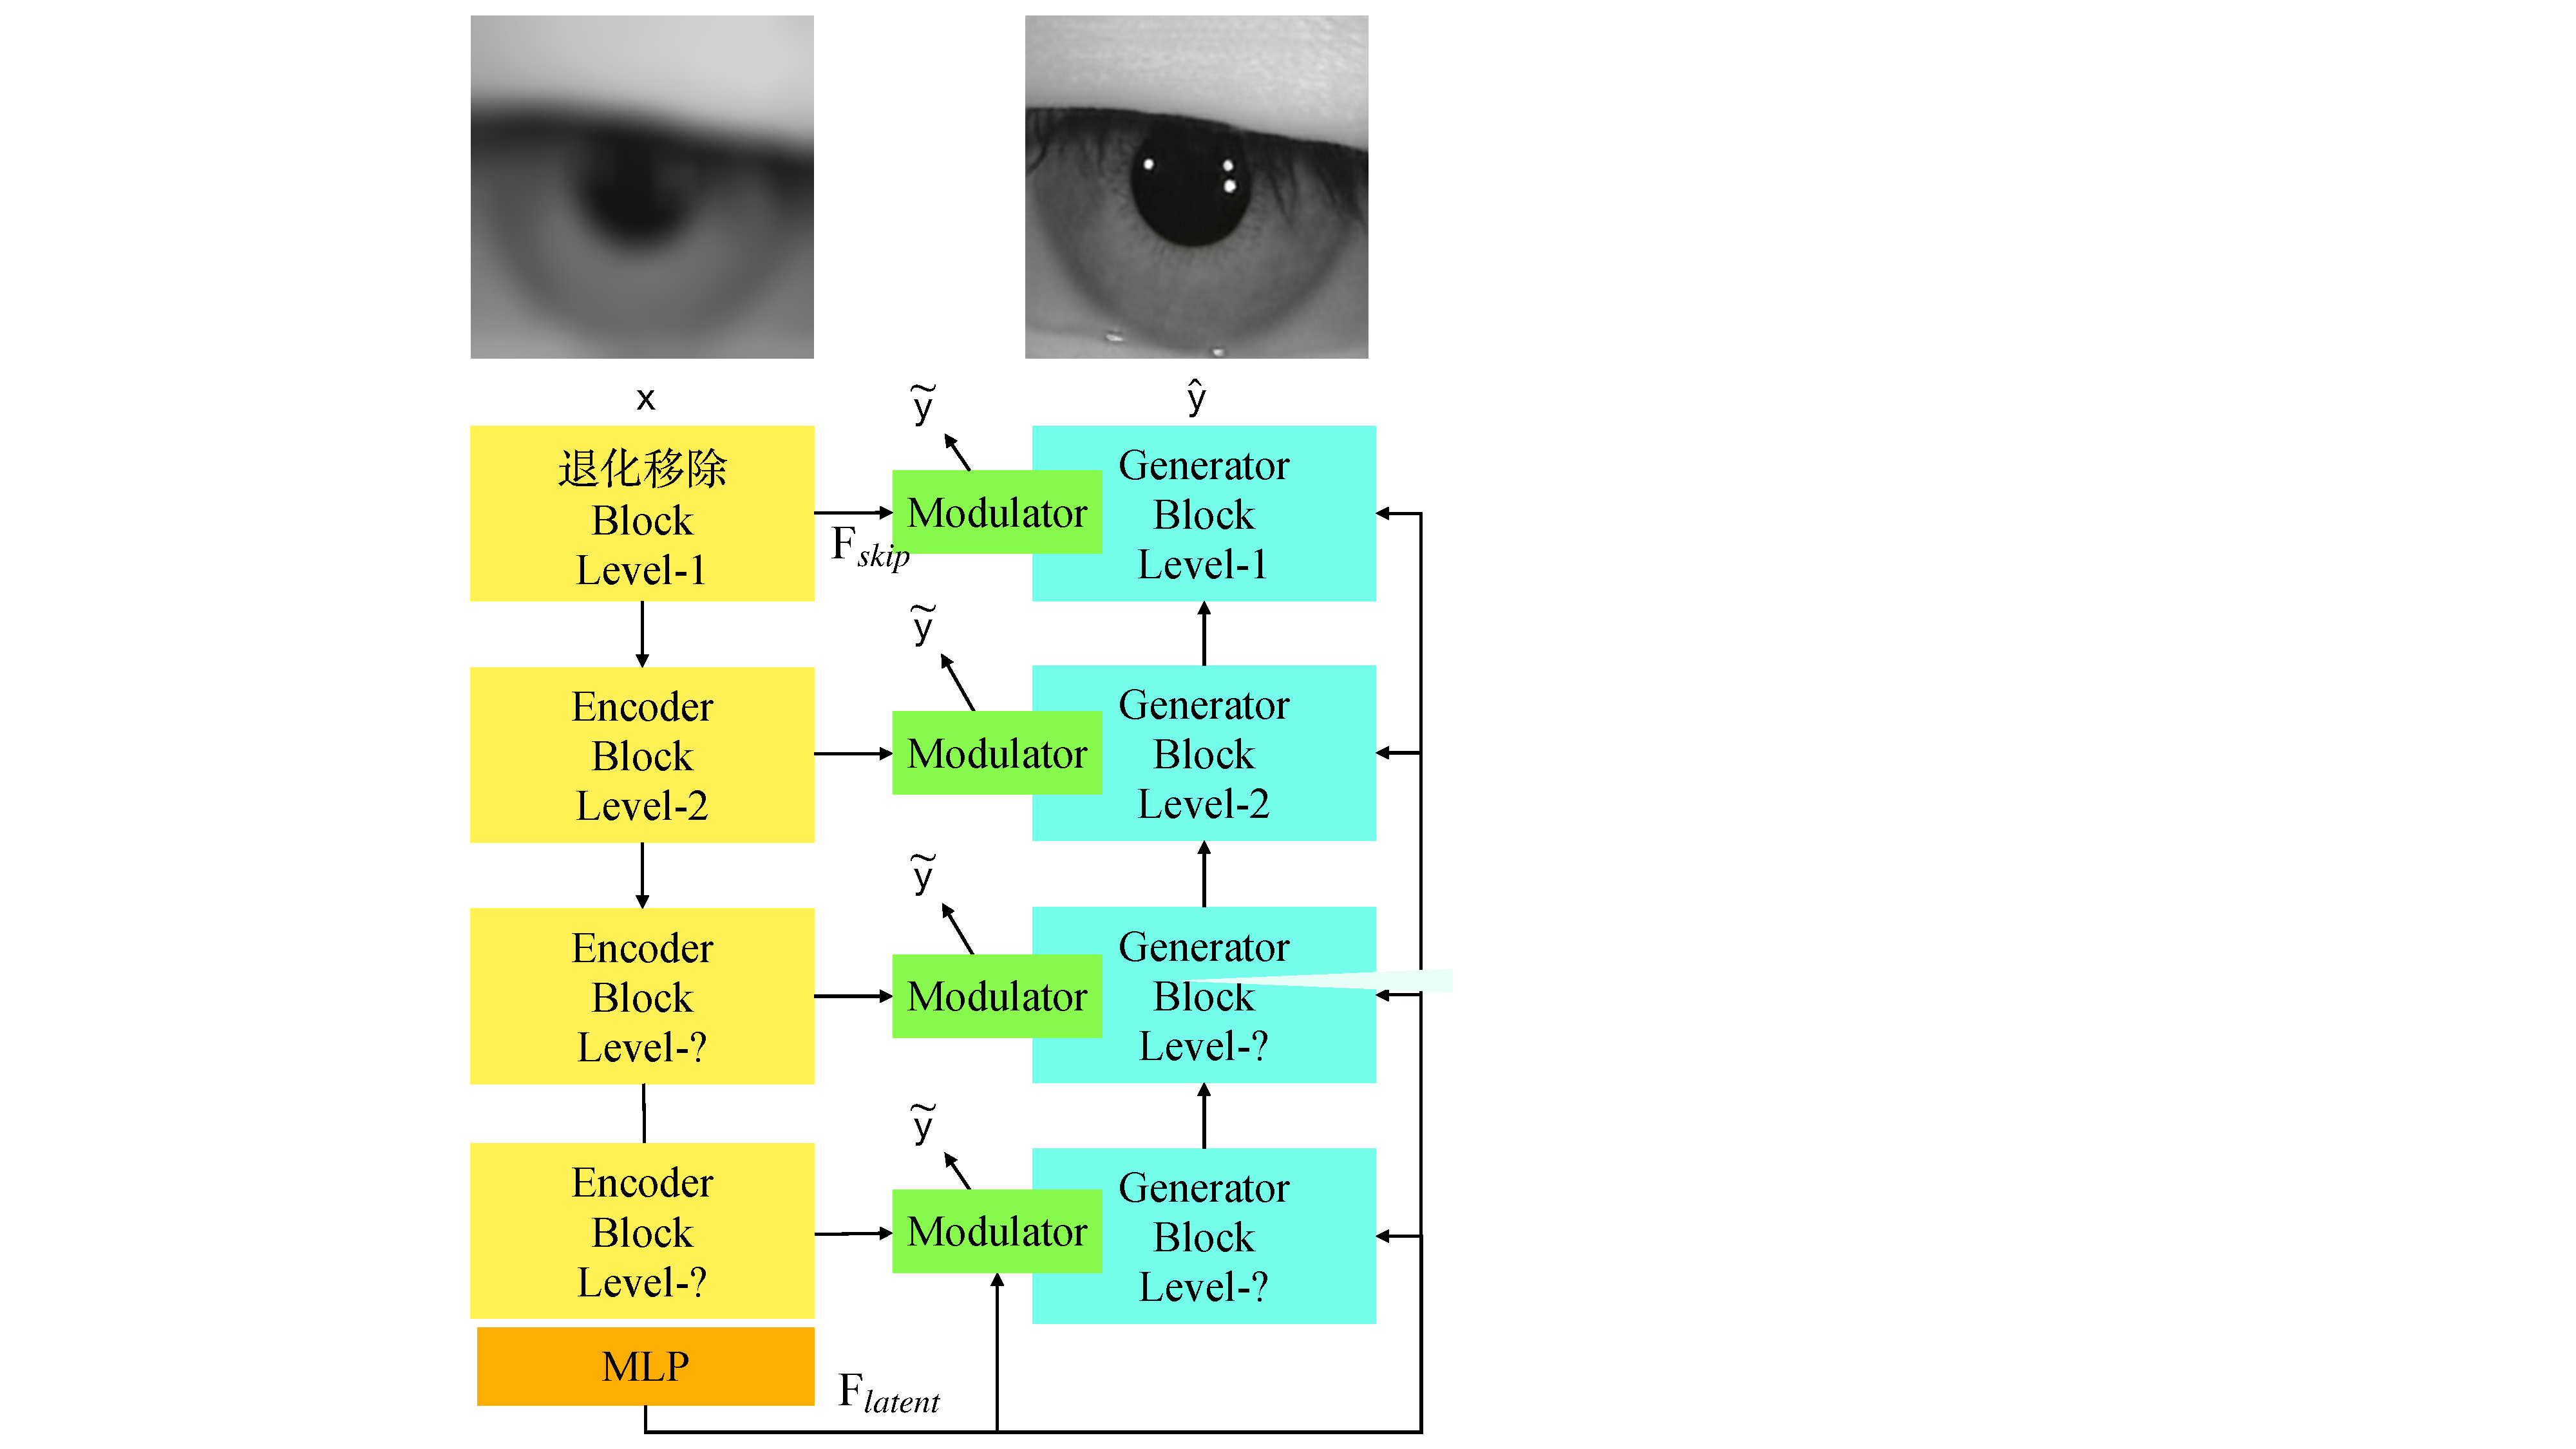
\includegraphics[width=4.5cm]{gipgan1.pdf}
	\end{textblock*}		

\end{frame}

%------------------------------------------------

\begin{frame}
	\frametitle{\large 基于生成式先验知识的虹膜图像修复方法}
	\framesubtitle{\normalsize 虹膜特征调制模块} % Optional subtitle

	\begin{varblock}[0.8\textwidth]{}
		为了嵌入虹膜生成式先验知识,本章设计了虹膜特征调制模块:
		\begin{enumerate}
			\item 将编码器的两个输出(跳跃特征图和隐向量)进行融合。
			\item 将生成器输出的特征在通道维度上平均分成两部分,一部分保持不变,另一部分进行调制,最后把这两部分连接在一起,就得到了最终的特征。
		\end{enumerate}		
	\end{varblock}	
	\begin{textblock*}{2.4cm}(13cm,1.7cm) % {block width} (coords)
		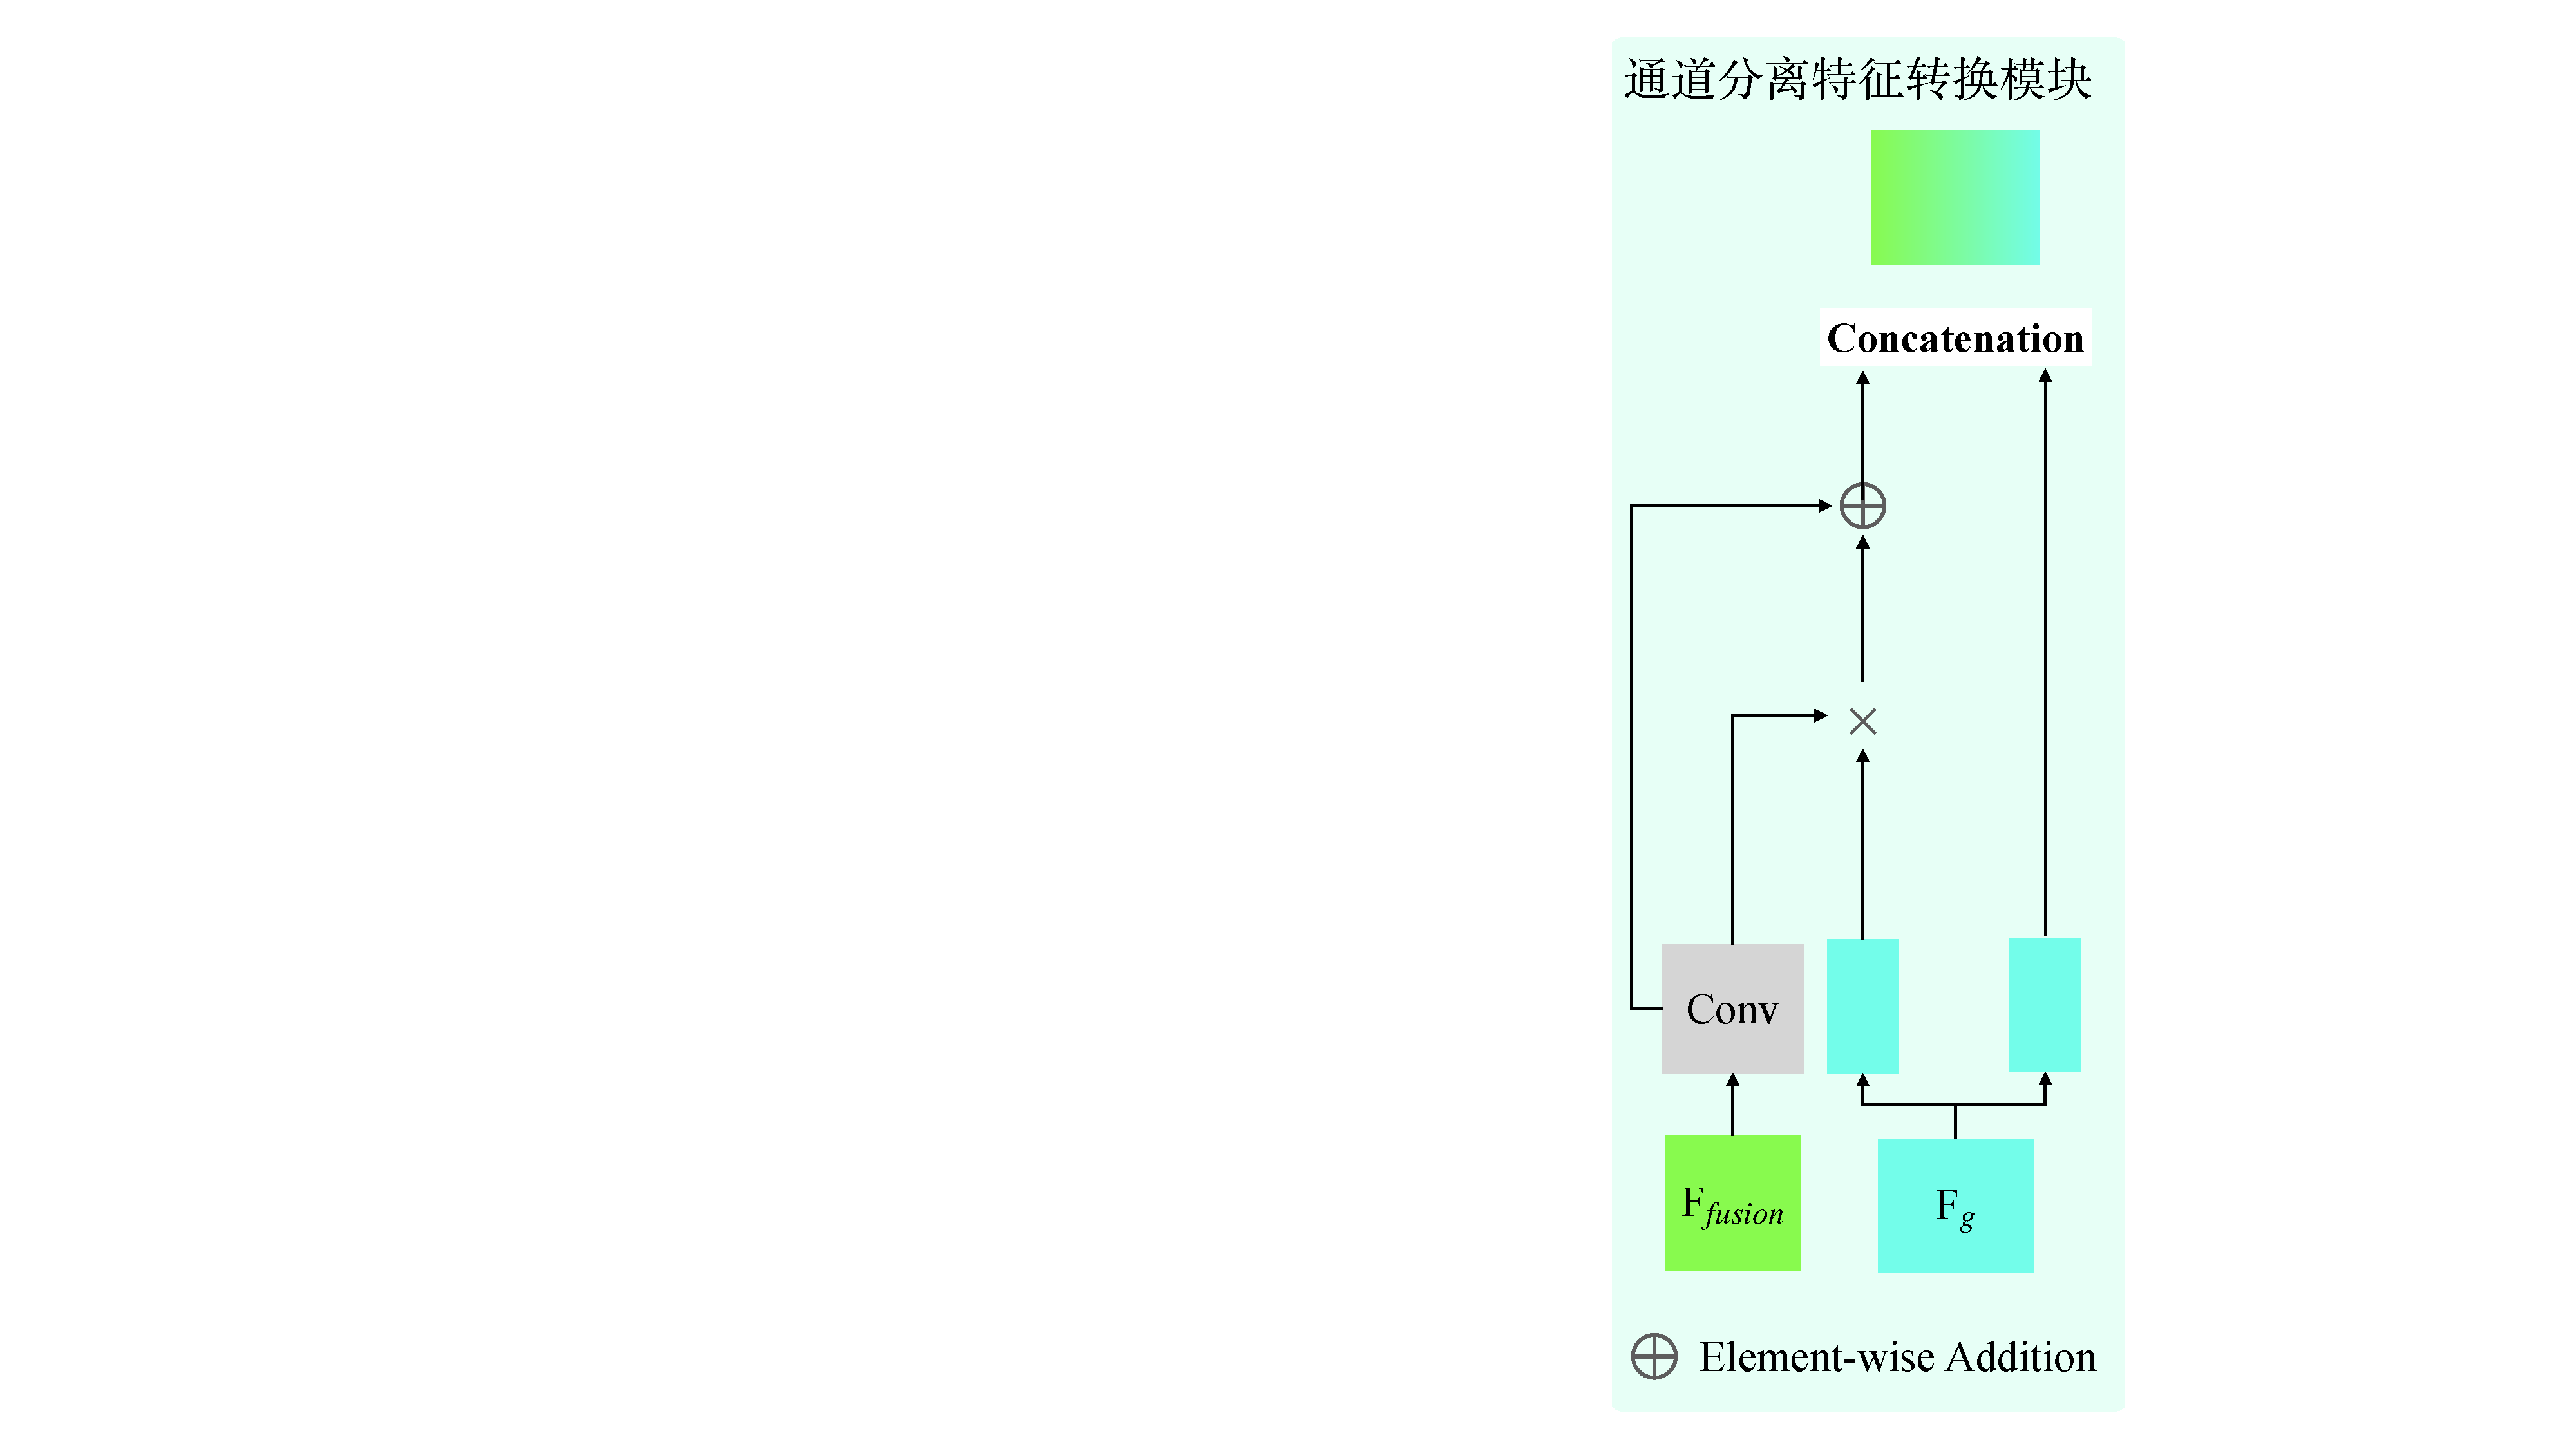
\includegraphics[width=2.4cm]{gipgan2.pdf}
	\end{textblock*}		

\end{frame}

%------------------------------------------------

\subsubsection{实验配置与结果}

%------------------------------------------------

\begin{frame}
	\frametitle{\large 基于生成式先验知识的虹膜图像修复方法}
	\framesubtitle{\normalsize 实验设置} % Optional subtitle
	\begin{varblock}[0.65\textwidth]{}
		\begin{itemize}
			\item 实验数据的处理与上一章相同。
			\item 采用的多层级网络结构的层级数为7,由浅到深每个层级输出图像分辨率分别为$[256^2, 128^2, 64^2, 32^2, 16^2, 8^2, 4^2]$。
			\item Adam优化器,学习率设为$2 \times 10^{-3}$。
			\item 深度学习框架为PyTorch。
			\item GPU型号为NVIDIA Tesla v100。
		\end{itemize}	
	\end{varblock}	

	\begin{textblock*}{5.5cm}(10.5cm,2cm) % {block width} (coords)
		
\includegraphics[width=5.5cm]{pytorch.jpg}
	\end{textblock*}	
	\begin{textblock*}{4cm}(11cm,4cm) % {block width} (coords)
		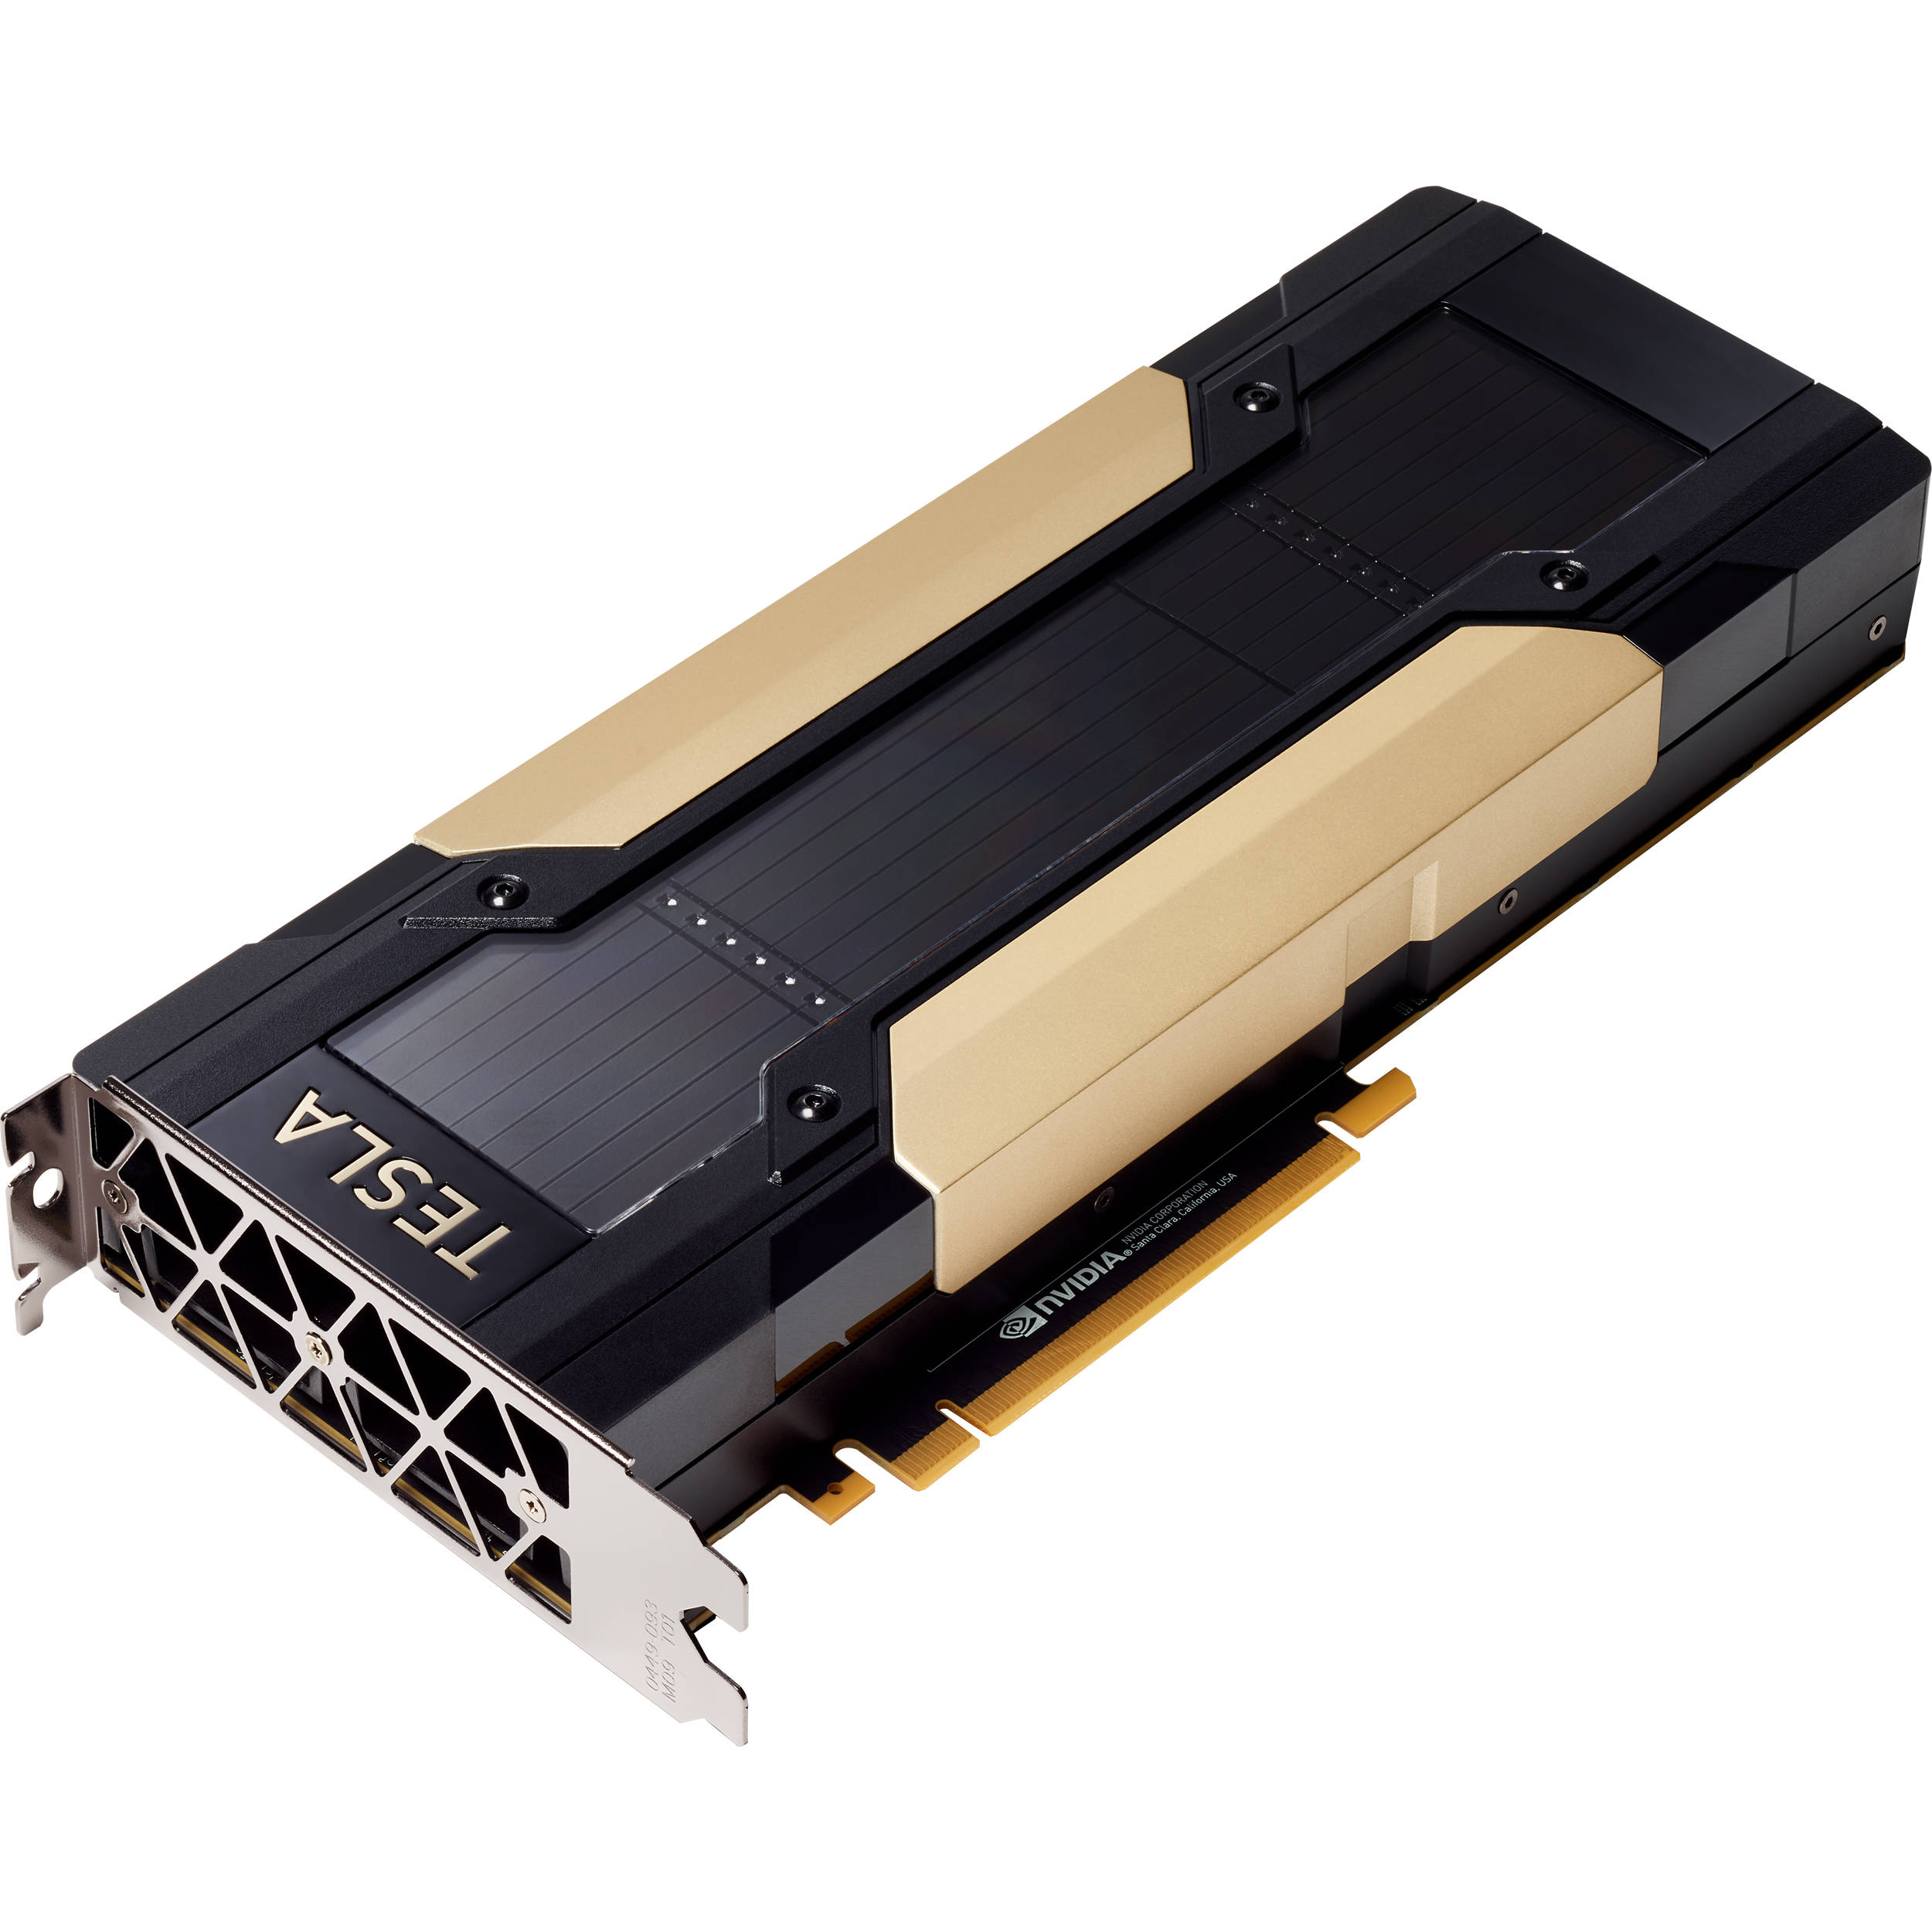
\includegraphics[width=4cm]{v100.jpg}
	\end{textblock*}	

\end{frame}

%------------------------------------------------

\begin{frame}
	\frametitle{定量实验结果}
	\framesubtitle{} % Optional subtitle
	
	\begin{table}
	\footnotesize
\begin{tabular}{ccc ccc ccc}
  \hline
  % after \\: \hline or \cline{col1-col2} \cline{col3-col4} ...
Method & AUC $\uparrow$ & EER $\downarrow$	& \makecell{TAR@FAR \\ =0.001 $\uparrow$} & \makecell{TAR@FAR \\ =0.01 $\uparrow$} & PSNR $\uparrow$ & SSIM $\uparrow$ & LPIPS $\downarrow$ \\ \hline
输入 & 0.9521 & 0.1153 & 0.1992 & 0.5361 & 30.68 & 0.8336 & 0.2865 \\
EDSR & 0.9796 & 0.0705 & 0.5356 & 0.7538 & \textbf{34.15} & \textbf{0.8808} & 0.1249 \\
RCAN & 0.9818 & 0.0679 & 0.5608 & 0.7666 & 33.57 & 0.8789 & 0.1324 \\
SRGAN & 0.9732 & 0.0853	& 0.3960 & 0.6705 & 32.85 & 0.8695 & 0.1311 \\
ESRGAN & 0.9585	& 0.1093 & 0.4816 & 0.6876 & 30.29 & 0.8314 & \textbf{0.1189} \\
SISN & 0.9836 & 0.0542 & 0.5878 & 0.8274 & 32.36 & 0.8729 & 0.1350 \\
\alert{本章方法} & \alert{0.9883} & \alert{0.0505} & \alert{0.7843} & \alert{0.8873} & 32.88 & 0.8631 & 0.1472 \\ \hline
原始图像 & 0.9914 & 0.0274 & 0.9323& 0.9613 & - & - & -\\ \hline
\end{tabular}
		\caption{基于生成式先验知识的虹膜图像修复方法与现有方法的定量结果对比。}
	\end{table}
\end{frame}

%------------------------------------------------

\begin{frame}
	\frametitle{定性实验结果}
	
	\begin{figure}
\centering
\begin{minipage}[t]{0.11\textwidth}
\centering

\includegraphics[width=1\linewidth]{cubic3.png}
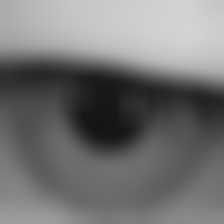
\includegraphics[width=1\linewidth]{cubic2.png}
\centerline{\footnotesize 输入}\medskip
\end{minipage}
\begin{minipage}[t]{0.11\textwidth}
\centering
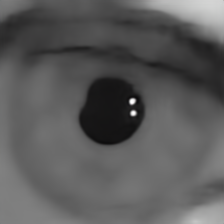
\includegraphics[width=1\linewidth]{edsr3.png}
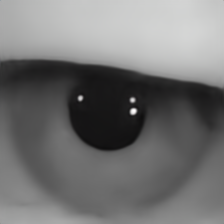
\includegraphics[width=1\linewidth]{edsr2.png}
\centerline{\footnotesize EDSR}\medskip
\end{minipage}
\begin{minipage}[t]{0.11\textwidth}
\centering
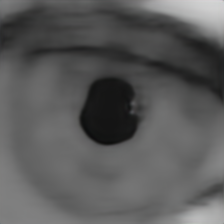
\includegraphics[width=1\linewidth]{rcan3.png}
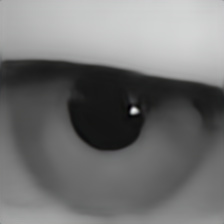
\includegraphics[width=1\linewidth]{rcan2.png}
\centerline{\footnotesize RCAN}\medskip
\end{minipage}
\begin{minipage}[t]{0.11\textwidth}
\centering
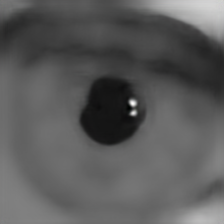
\includegraphics[width=1\linewidth]{srgan3.png}
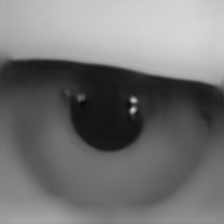
\includegraphics[width=1\linewidth]{srgan2.png}
\centerline{\footnotesize SRGAN}\medskip
\end{minipage}
\begin{minipage}[t]{0.11\textwidth}
\centering
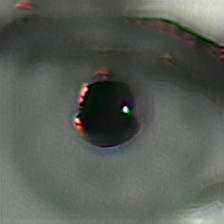
\includegraphics[width=1\linewidth]{esrgan3.png}
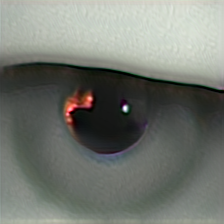
\includegraphics[width=1\linewidth]{esrgan2.png}
\centerline{\footnotesize ESRGAN}\medskip
\end{minipage}
\begin{minipage}[t]{0.11\textwidth}
\centering
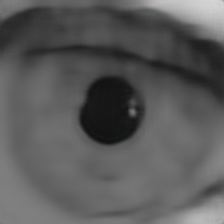
\includegraphics[width=1\linewidth]{sisn_S2309L07_HR.png}
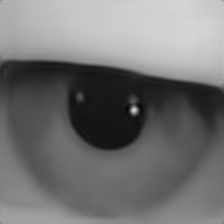
\includegraphics[width=1\linewidth]{sisn_S2308L02_HR.png}
\centerline{\footnotesize SISN}\medskip
\end{minipage}
\begin{minipage}[t]{0.11\textwidth}
\centering
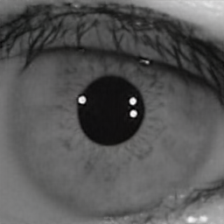
\includegraphics[width=1\linewidth]{S2309L07_gipgan.png}
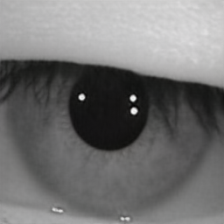
\includegraphics[width=1\linewidth]{S2308L02_gipgan.png}
\centerline{\footnotesize \alert{本章方法}}\medskip
\end{minipage}
\begin{minipage}[t]{0.11\textwidth}
\centering
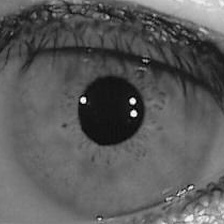
\includegraphics[width=1\linewidth]{gt3.png}
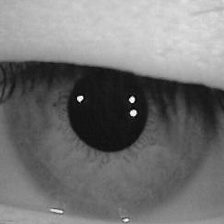
\includegraphics[width=1\linewidth]{gt2.png}
\centerline{\footnotesize 原始图像}\medskip
\end{minipage}
\caption{基于生成式先验知识的虹膜图像修复方法与现有方法的定性实验结果对比。}
	\end{figure}
\end{frame}

%------------------------------------------------

\begin{frame}
	\frametitle{虹膜识别性能测试}
	\begin{figure}
\centering
% \centerline{\epsfig{figure=image1.ps,width=8.5cm}}
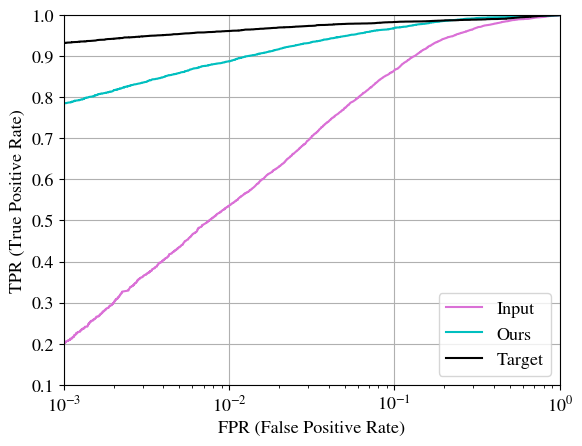
\includegraphics[width=0.5\textwidth]{roc_gipgan.png}
\caption{基于生成式先验知识的虹膜图像修复方法的ROC曲线。}
	\end{figure}
\end{frame}

%------------------------------------------------

\begin{frame}
	\frametitle{消融实验}
	\framesubtitle{} % Optional subtitle
	
	\begin{table}
	\footnotesize
\begin{tabular}{ccc ccc ccc}
  \hline
  % after \\: \hline or \cline{col1-col2} \cline{col3-col4} ...
Method & AUC $\uparrow$ & EER $\downarrow$	& \makecell{TAR@FAR \\ =0.001 $\uparrow$} & \makecell{TAR@FAR \\ =0.01 $\uparrow$} & PSNR $\uparrow$ & SSIM $\uparrow$ \\ \hline
w/o Generative Iris Prior & 0.9513 & 0.1273 & 0.5145 & 0.6678 & 29.43 & 0.8023  \\
w/o Chanel-Split & 0.9903 & 0.0435 & 0.7889 & 0.9060 & 32.96 & 0.8734  \\
w/o SFT & 0.9879 & 0.0480 & 0.7721 & 0.8917 & 32.12 & 0.8582  \\
本章方法 & 0.9883 & 0.0505 & 0.7843 & 0.8873 & 32.88 & 0.8631 \\ \hline
\end{tabular}
		\caption{基于生成式先验知识的虹膜图像修复方法的消融实验结果。}
	\end{table}
\end{frame}

%------------------------------------------------

\section{总结与展望}

\begin{frame}
	\frametitle{工作总结}
	\begin{varblock}[1\textwidth]{}
		\small 	传统自注意力机制的计算复杂度随着图片分辨率的增大而以平方的速度增长。这导致Transformer无法有效地应用到高分辨率的图像修复任务中。本文采用了作用于通道维度的自注意力机制,它拥有线性的计算复杂度,使得Transformer在图像修复任务中的应用变得更加切实可行。	
	\end{varblock}		
	\begin{varblock}[1\textwidth]{}
		\small 	传统的激活网络以完全相同的方法独立地处理每个像素上的信息。本文设计了深度级激活网络,不仅具有从相邻像素编码信息的能力,还可以有效地学习到图像局部的结构,丰富了图像中的细节。	
	\end{varblock}				
	\begin{varblock}[1\textwidth]{}
		\small 	传统的图像质量增强方法使用生成对抗网络直接生成最终图像,没有利用图像的特性。本文设计了虹膜特征调制模块,嵌入了虹膜生成式先验知识,使得输出图像的纹理更加真实。	
	\end{varblock}		
\end{frame}

%------------------------------------------------

\begin{frame}
	\frametitle{工作展望}
	\begin{varblock}[1\textwidth]{}
	 	\small 本文的方法中,如果去掉金字塔损失,识别性能上升,图像质量下降。金字塔损失由L1损失构成。后续若想进一步提升识别性能,需减少对L1损失的使用。	
	\end{varblock}		
	
	\begin{varblock}[1\textwidth]{}
%		\setstretch{1}
	 	\small 本文的方法中,如果不使用通道分离特征转:不是原始方法中对一半通道进行特征转换,而是对所有通道进行特征转换,会使计算复杂度增大,识别性能和图像质量上升。后续若想要进一步提升识别性能,可以将所有通道进行特征转换。
	\end{varblock}		
				
	\begin{varblock}[1\textwidth]{}
	 	\small 本文的方法参数量较大,适合部署在算力较强的平台上。近年来,为了提升计算效率,具有多种处理器或内核(如CPU、GPU、ASIC、FGA和NPU)的系统被越来越广泛地使用。为了适应这一趋势,基于深度学习的图像质量增强方法还需要增强其可扩缩性。例如,根据不同平台的算力、不同的数据、每张图像中的不同区域,智能地调节方法中使用到的网络层级数目,从而在性能与效率之间寻求最优平衡。
	\end{varblock}	
	
%\begin{tikzpicture}[remember picture,overlay]
%\node[anchor=north east] at ($(current page.north east)+(-1cm,-1.5cm)$){\begin{tabular}{|c|c|}\hline                                             
%0&0\\\hline                                                              
%0&0\\\hline                                                              
%1&1\\\hline                                                              
%0&0\\\hline                                                              
%0&1\\\hline                                                              
%1&0\\\hline                                                              
%\end{tabular}};
%\end{tikzpicture}

\end{frame}
%------------------------------------------------

\begin{frame}
	\frametitle{工作展望}	
\begin{table}
	\footnotesize
\begin{tabular}{ccc ccc ccc}
  \hline
  % after \\: \hline or \cline{col1-col2} \cline{col3-col4} ...
Method & \#Parameters $\downarrow$ & \makecell{Inference \\ Time $\downarrow$}\\ \hline
EDSR & 43M & 88ms\\
RCAN & 16M & 70ms \\
SRGAN & \textbf{1M} & \textbf{10ms} \\
ESRGAN &  17M & 154ms \\
DeblurGANv2 &  11M & \underline{15ms} \\
HiFaceGAN & 161M & 91ms \\
SISN & \underline{8M} & 202ms \\
SparNet & 11M & 134ms \\
\textbf{本文的两种方法} & 70M & 150ms \\ \hline
\end{tabular}
		\caption{本文的方法与现有方法参数量和推理时间的对比。}
	\end{table}
\end{frame}

%------------------------------------------------

\begin{frame}
	\frametitle{攻读学位期间发表的学术论文}
[1] \alert{Huang Yubo}, Wang Jia, Li Peipei, Xiang Liuyu, Li Peigang, He Zhaofeng. Generative Iris Prior Embedded Transformer for Iris Restoration [A]. // 2023 IEEE International Conference on Multimedia and Expo (ICME) [C]. Los Alamitos: IEEE Computer Society, 2023: 1–6. (\alert{CCF-B}, in press).
\end{frame}


%----------------------------------------------------------------------------------------
%	CLOSING SLIDE
%----------------------------------------------------------------------------------------

\begin{frame}[plain] % The optional argument 'plain' hides the headline and footline
	\begin{center}
		{\Huge \textbf{谢谢}}
		
		\bigskip\bigskip % Vertical whitespace
		
		{\LARGE 欢迎各位老师指正!}
	\end{center}
\end{frame}

%----------------------------------------------------------------------------------------

\end{document} 